%% ─── Introducción ──────────────────────────────────────────────────────────
\section{Introducción}

En instalaciones eléctricas residenciales, la topología de conexión de las luminarias determina la tensión que recibe cada punto de luz, la corriente que debe conducir el circuito ramal y la independencia operativa de cada elemento. Aunque este principio es fundamental en ingeniería eléctrica, en proyectos de pequeña escala suele obviarse el análisis formal, imponiéndose la práctica constructiva sobre el rigor técnico.

Este artículo documenta el diseño, análisis y simulación del sistema de iluminación del proyecto de vivienda unifamiliar en Curiti, Vereda Líbano (Santander, Colombia), edificación de cuatro niveles proyectados sobre un lote de 98~m². Se evalúan dos topologías de circuito —serie y paralelo— y dos esquemas de mando —control manual con interruptores unipolares y control automático con relés por detección de presencia— contrastando en cada caso los resultados analíticos con los obtenidos en simulación.

La validación se realizó en SimulIDE. Dado que las luminarias modeladas son cargas puramente resistivas, la acometida posterior al medidor se representó como fuente de tensión continua de 120~V~CD, criterio válido para análisis en régimen permanente resistivo \cite{hayt2012}.

Los objetivos del estudio son: (i)~elaborar los planos arquitectónico y eléctrico con simbología IEC/ANSI; (ii)~calcular las variables eléctricas de ambas topologías; (iii)~simular los cuatro escenarios en SimulIDE; y (iv)~formular una recomendación técnica para la instalación futura.

%% ─── Justificación ──────────────────────────────────────────────────────────
\section{Justificación}

La selección incorrecta de la topología de un circuito de alumbrado tiene consecuencias directas sobre la calidad del servicio. En serie, la apertura de filamento en una sola lámpara interrumpe todo el ramal; además, la tensión se distribuye entre los elementos y ninguno recibe su valor nominal. En paralelo, en cambio, cada rama es independiente y opera siempre a la tensión de diseño.

Más allá del caso particular, el ejercicio permite aplicar las leyes de Kirchhoff y la Ley de Ohm a un escenario con geometría y condiciones de alimentación definidas, desarrollando competencias de diseño, cálculo y simulación transferibles a proyectos de mayor escala.

%% ─── Marco teórico ──────────────────────────────────────────────────────────
\section{Marco teórico}

\subsection{Leyes fundamentales}

La Ley de Ohm, $V = I \cdot R$, relaciona la tensión, la corriente y la resistencia de un elemento. Las Leyes de Kirchhoff complementan el modelo: la LCK establece $\sum I_{\text{ent}} = \sum I_{\text{sal}}$ en cada nodo, y la LTK indica $\sum V = 0$ en toda malla cerrada \cite{nilsson2015}. La potencia disipada se obtiene como $P = V \cdot I = I^2 R = V^2 / R$.

\subsection{Conexión en serie}

En serie, todos los elementos comparten la misma corriente. La resistencia equivalente y la tensión por elemento son:
\begin{equation}
  R_{eq,s} = n \cdot R, \qquad V_k = \frac{V_s}{n}
  \label{eq:serie}
\end{equation}
La división de tensión reduce la potencia de cada lámpara y la falla de un elemento apaga el ramal completo.

\subsection{Conexión en paralelo}

En paralelo, todos los elementos quedan sometidos a la tensión de la fuente:
\begin{equation}
  R_{eq,p} = \frac{R}{n}, \qquad I_{total} = n \cdot \frac{V_s}{R}
  \label{eq:paralelo}
\end{equation}
Cada lámpara opera a potencia nominal y es eléctricamente independiente de las demás. Esta es la topología prescrita por el RETIE \cite{retie2013} y la NTC~2050 \cite{ntc2050} para instalaciones residenciales en Colombia.

\subsection{Modelado de la fuente y contexto normativo}

La acometida residencial en Colombia es 120~V~CA a 60~Hz. Para cargas puramente resistivas, los valores eficaces (RMS) producen los mismos efectos de potencia que una fuente CD de igual magnitud, por lo que el circuito se modela con 120~V~CD, conforme a la práctica habitual en análisis de régimen permanente \cite{hayt2012}.

El RETIE exige que los circuitos ramales de iluminación operen en paralelo, con protección termomagnética individual por ramal y conductor dimensionado para la corriente de diseño. La NTC~2050 fija en 15~A o 20~A la capacidad máxima de los circuitos de alumbrado residencial.

\subsection{SimulIDE como herramienta de validación}

SimulIDE es un simulador de circuitos de código abierto que resuelve ecuaciones nodales en tiempo real. Soporta resistencias, fuentes, interruptores y relés, permitiendo implementar tanto el mando manual como el automático. Aunque su motor es más sencillo que LTspice o Multisim, es suficiente para validar circuitos resistivos en régimen permanente \cite{simulide}.

%% ─── Metodología ────────────────────────────────────────────────────────────
\section{Metodología}

El proyecto se desarrolló en cuatro fases:

\begin{enumerate}
  \item \textbf{Levantamiento}: revisión de planos arquitectónicos del proyecto y verificación de cotas en el lote (actualmente vacío) con cinta métrica.

  \item \textbf{Diseño}: elaboración del plano arquitectónico en AutoCAD (14~m~$\times$~7~m, cuatro plantas) y esquema eléctrico unifilar para cada topología con simbología IEC~60617. Se definieron 44~puntos de iluminación por criterio de densidad luminosa ($\approx 1$ luminaria cada 6~m², mínimo una por recinto), modelando cada una como $R = 240~\Omega$.

  \item \textbf{Simulación}: implementación en SimulIDE de cuatro escenarios: paralelo con mando manual, paralelo con mando automático, serie con mando manual y serie con mando automático.

  \item \textbf{Análisis}: contraste entre resultados analíticos y de simulación, elaboración de tablas y recomendaciones.
\end{enumerate}

%% ─── Desarrollo del diseño ──────────────────────────────────────────────────
\section{Diseño eléctrico}

\subsection{Descripción del proyecto}

La vivienda proyectada se localiza en Curiti, Vereda Líbano, Santander. El lote es de 14~m~$\times$~7~m (98~m²); el área construida varía por planta debido a terrazas, azoteas y jardín. La Tabla~\ref{tab:medidas} resume los parámetros generales.

\begin{table}[H]
\centering
\caption{Parámetros generales del proyecto.}
\label{tab:medidas}
\begin{tabular}{lc}
\toprule
\textbf{Parámetro} & \textbf{Valor} \\
\midrule
Frente del lote          & 7{,}00 m \\
Fondo del lote           & 14{,}00 m \\
Área de terreno          & 98{,}00 m² \\
Plantas proyectadas      & 4 \\
Total de luminarias      & 44 \\
$R$ por luminaria        & 240~$\Omega$ \\
$V_s$ (modelo CD)        & 120~V \\
\bottomrule
\end{tabular}
\end{table}

\subsection{Inventario de luminarias}

La Tabla~\ref{tab:inventario} presenta el inventario completo de luminarias por planta y ambiente, con las dimensiones relevadas en plano y el criterio de asignación aplicado.

% Tabla ancha → table* para ocupar ambas columnas
\begin{table*}[H]
\centering
\caption{Inventario de luminarias por planta y ambiente.}
\label{tab:inventario}
\begin{tabular}{llcccc}
\toprule
\textbf{Planta} & \textbf{Ambiente} & \textbf{Ancho (m)} & \textbf{Largo (m)} & \textbf{Área (m²)} & \textbf{N° Lum.} \\
\midrule
\multirow{13}{*}{Primer Piso}
 & Estacionamiento          & 7{,}0 & 4{,}5 & 31{,}50 & 2 \\
 & Hall – Ingreso           & 3{,}0 & 2{,}5 &  7{,}50 & 1 \\
 & Sala                     & 4{,}0 & 3{,}5 & 14{,}00 & 2 \\
 & Comedor                  & 3{,}5 & 3{,}0 & 10{,}50 & 2 \\
 & Cocina                   & 2{,}5 & 2{,}5 &  6{,}25 & 1 \\
 & Patio de Servicio        & 2{,}0 & 2{,}0 &  4{,}00 & 1 \\
 & Dormitorio Principal     & 3{,}5 & 3{,}5 & 12{,}25 & 2 \\
 & Baño                     & 2{,}0 & 1{,}5 &  3{,}00 & 1 \\
 & Dormitorio               & 3{,}0 & 3{,}0 &  9{,}00 & 1 \\
 & Estudio                  & 3{,}0 & 2{,}5 &  7{,}50 & 1 \\
 & Terraza                  & 3{,}5 & 2{,}0 &  7{,}00 & 1 \\
 & Jardín                   & 3{,}0 & 2{,}5 &  7{,}50 & 1 \\
 & Cisterna / Terraza ext   & 2{,}5 & 2{,}0 &  5{,}00 & 1 \\
\midrule
\multirow{8}{*}{Segundo Piso}
 & Dormitorio Principal     & 3{,}5 & 3{,}5 & 12{,}25 & 2 \\
 & Dormitorio               & 3{,}0 & 3{,}0 &  9{,}00 & 2 \\
 & Baño                     & 2{,}0 & 1{,}5 &  3{,}00 & 1 \\
 & Sala                     & 4{,}0 & 3{,}5 & 14{,}00 & 2 \\
 & Comedor                  & 3{,}5 & 3{,}0 & 10{,}50 & 2 \\
 & Cocina                   & 2{,}5 & 2{,}5 &  6{,}25 & 2 \\
 & Escalera                 & 2{,}0 & 2{,}0 &  4{,}00 & 1 \\
 & Pozo de Luz              & 2{,}0 & 2{,}0 &  4{,}00 & 2 \\
\midrule
\multirow{9}{*}{Tercer Piso}
 & Sala de Estar / Juegos / TV & 5{,}0 & 4{,}0 & 20{,}00 & 2 \\
 & Bar                      & 2{,}5 & 2{,}0 &  5{,}00 & 1 \\
 & Dormitorio de Servicio   & 3{,}0 & 2{,}5 &  7{,}50 & 1 \\
 & Baño                     & 2{,}0 & 1{,}5 &  3{,}00 & 1 \\
 & Azotea                   & 4{,}0 & 3{,}5 & 14{,}00 & 1 \\
 & Patio de Servicio        & 2{,}0 & 2{,}0 &  4{,}00 & 1 \\
 & Pozo de Luz              & 2{,}0 & 2{,}0 &  4{,}00 & 1 \\
 & Balcón                   & 3{,}5 & 1{,}5 &  5{,}25 & 1 \\
 & Escalera                 & 2{,}0 & 2{,}0 &  4{,}00 & 0 \\
\midrule
\multirow{3}{*}{Planta Techos}
 & Techos (área cubierta)   & 7{,}0 & 10{,}0 & 70{,}00 & 2 \\
 & Proyección Tanque        & 2{,}0 &  2{,}0 &  4{,}00 & 1 \\
 & Escalera de Gato         & 1{,}0 &  1{,}0 &  1{,}00 & 1 \\
\midrule
\textbf{TOTAL} & & & & \textbf{98{,}00} & \textbf{44} \\
\bottomrule
\end{tabular}
\end{table*}

\subsection{Planos arquitectónicos}

Los planos (Figuras~\ref{fig:plano_p1}--\ref{fig:plano_techos}) se elaboraron en AutoCAD respetando las cotas del proyecto. Sobre ellos se superpusieron los símbolos de luminaria, interruptor y conductor conforme a IEC~60617.

\begin{figure}[H]
\centering
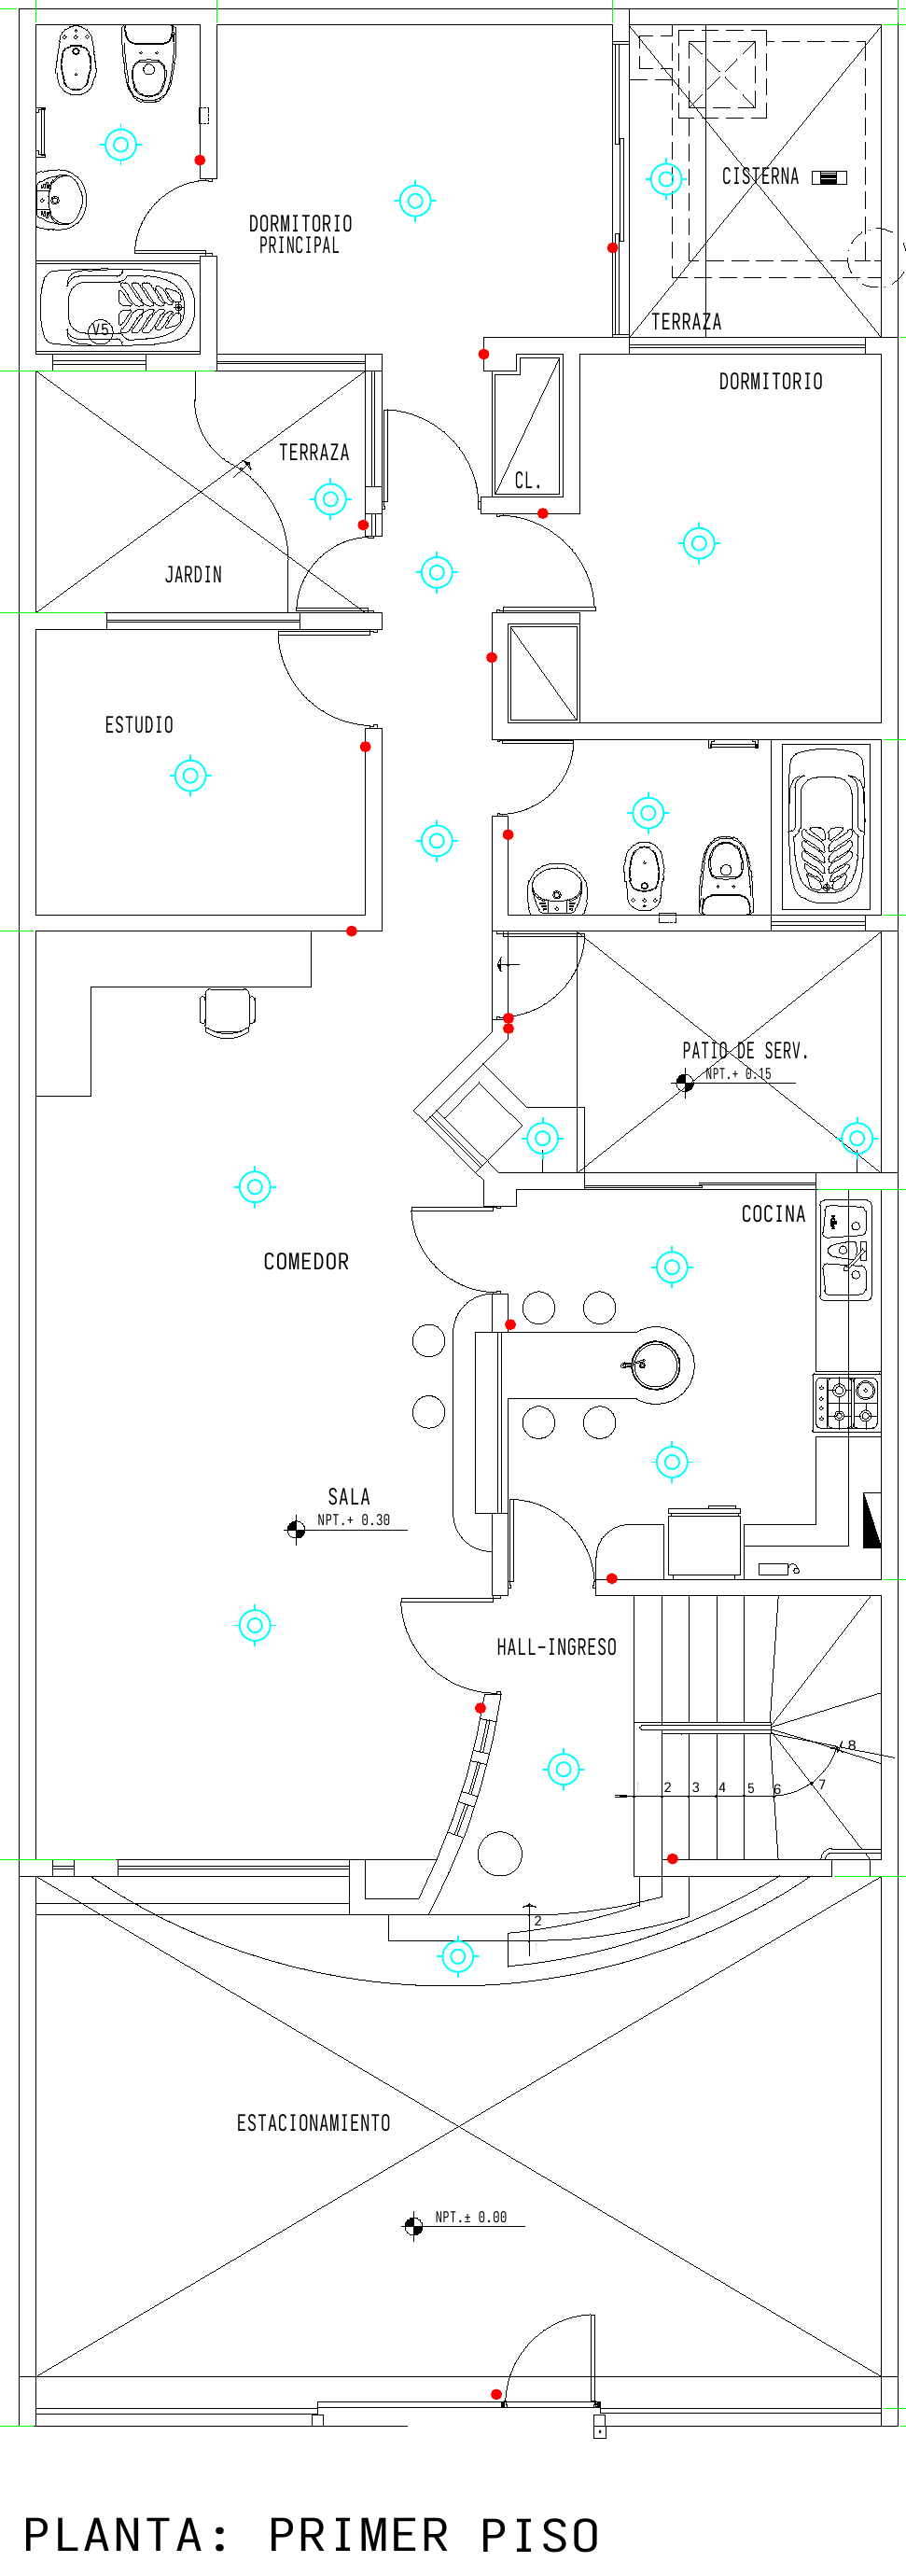
\includegraphics[width=0.85\linewidth]{images/PlanoArquitectonico-1piso.png}
\caption{Plano — Primer piso (17 luminarias).}
\label{fig:plano_p1}
\end{figure}

\begin{figure}[H]
\centering
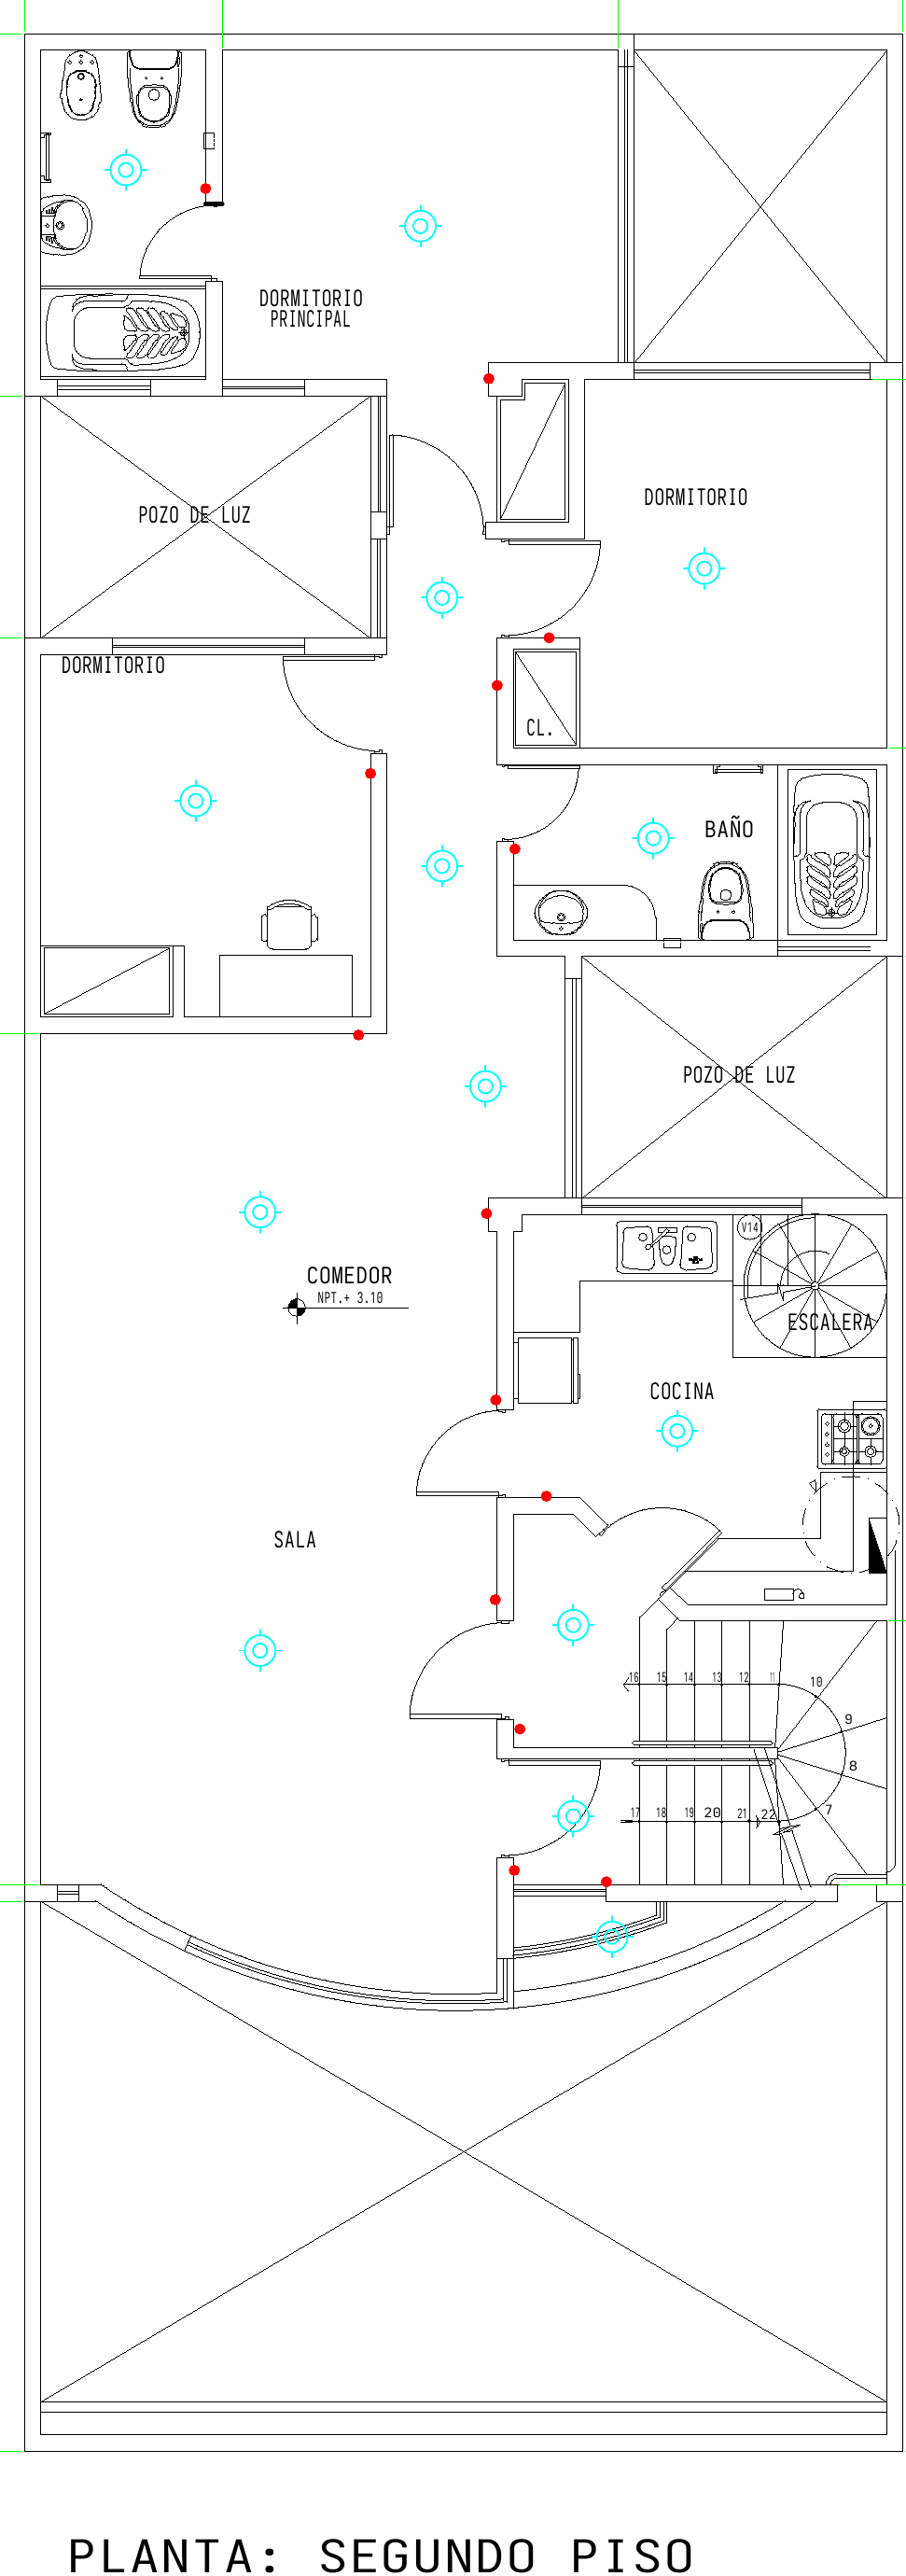
\includegraphics[width=0.85\linewidth]{images/PlanoArquitectonico-2piso.png}
\caption{Plano — Segundo piso (14 luminarias).}
\label{fig:plano_p2}
\end{figure}

\begin{figure}[H]
\centering
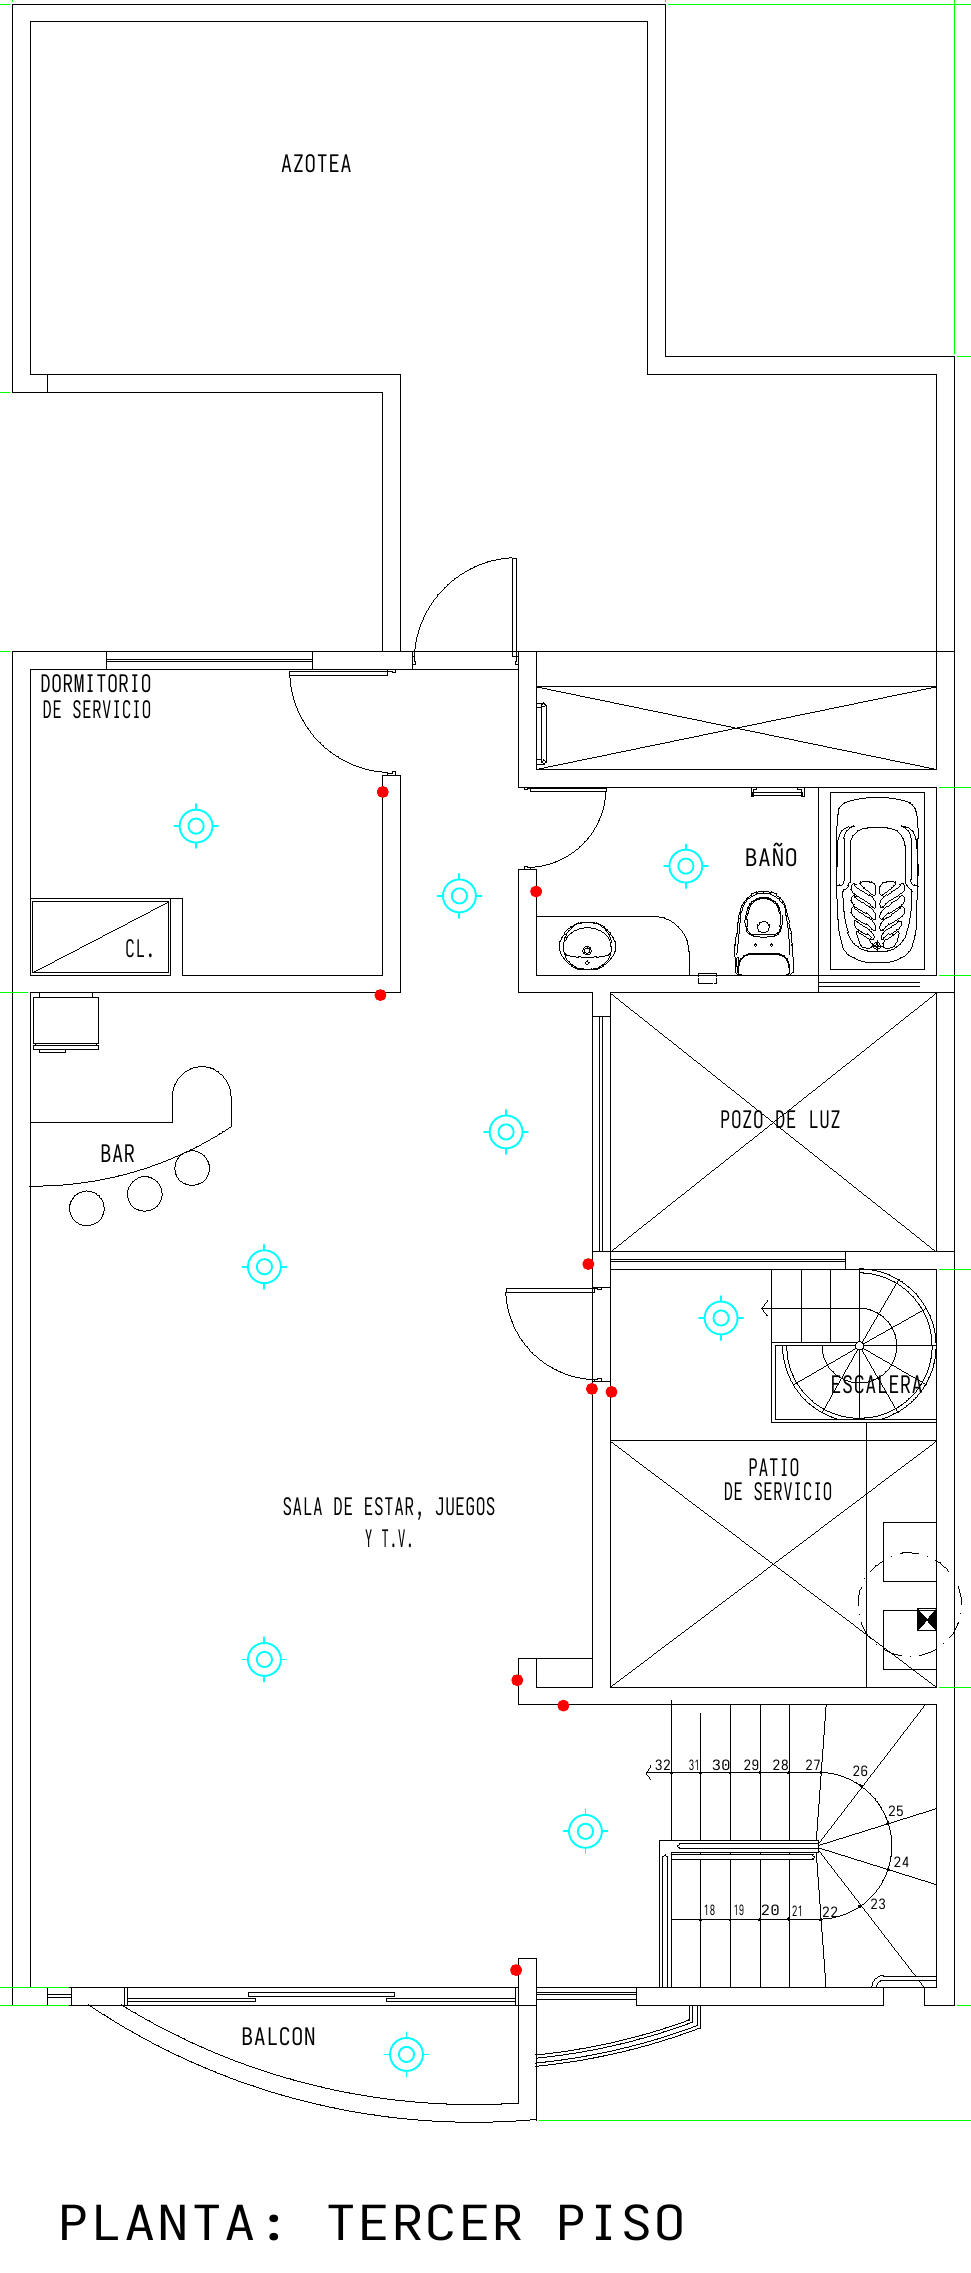
\includegraphics[width=0.85\linewidth]{images/PlanoArquitectonico-3piso.png}
\caption{Plano — Tercer piso (9 luminarias).}
\label{fig:plano_p3}
\end{figure}

\begin{figure}[H]
\centering
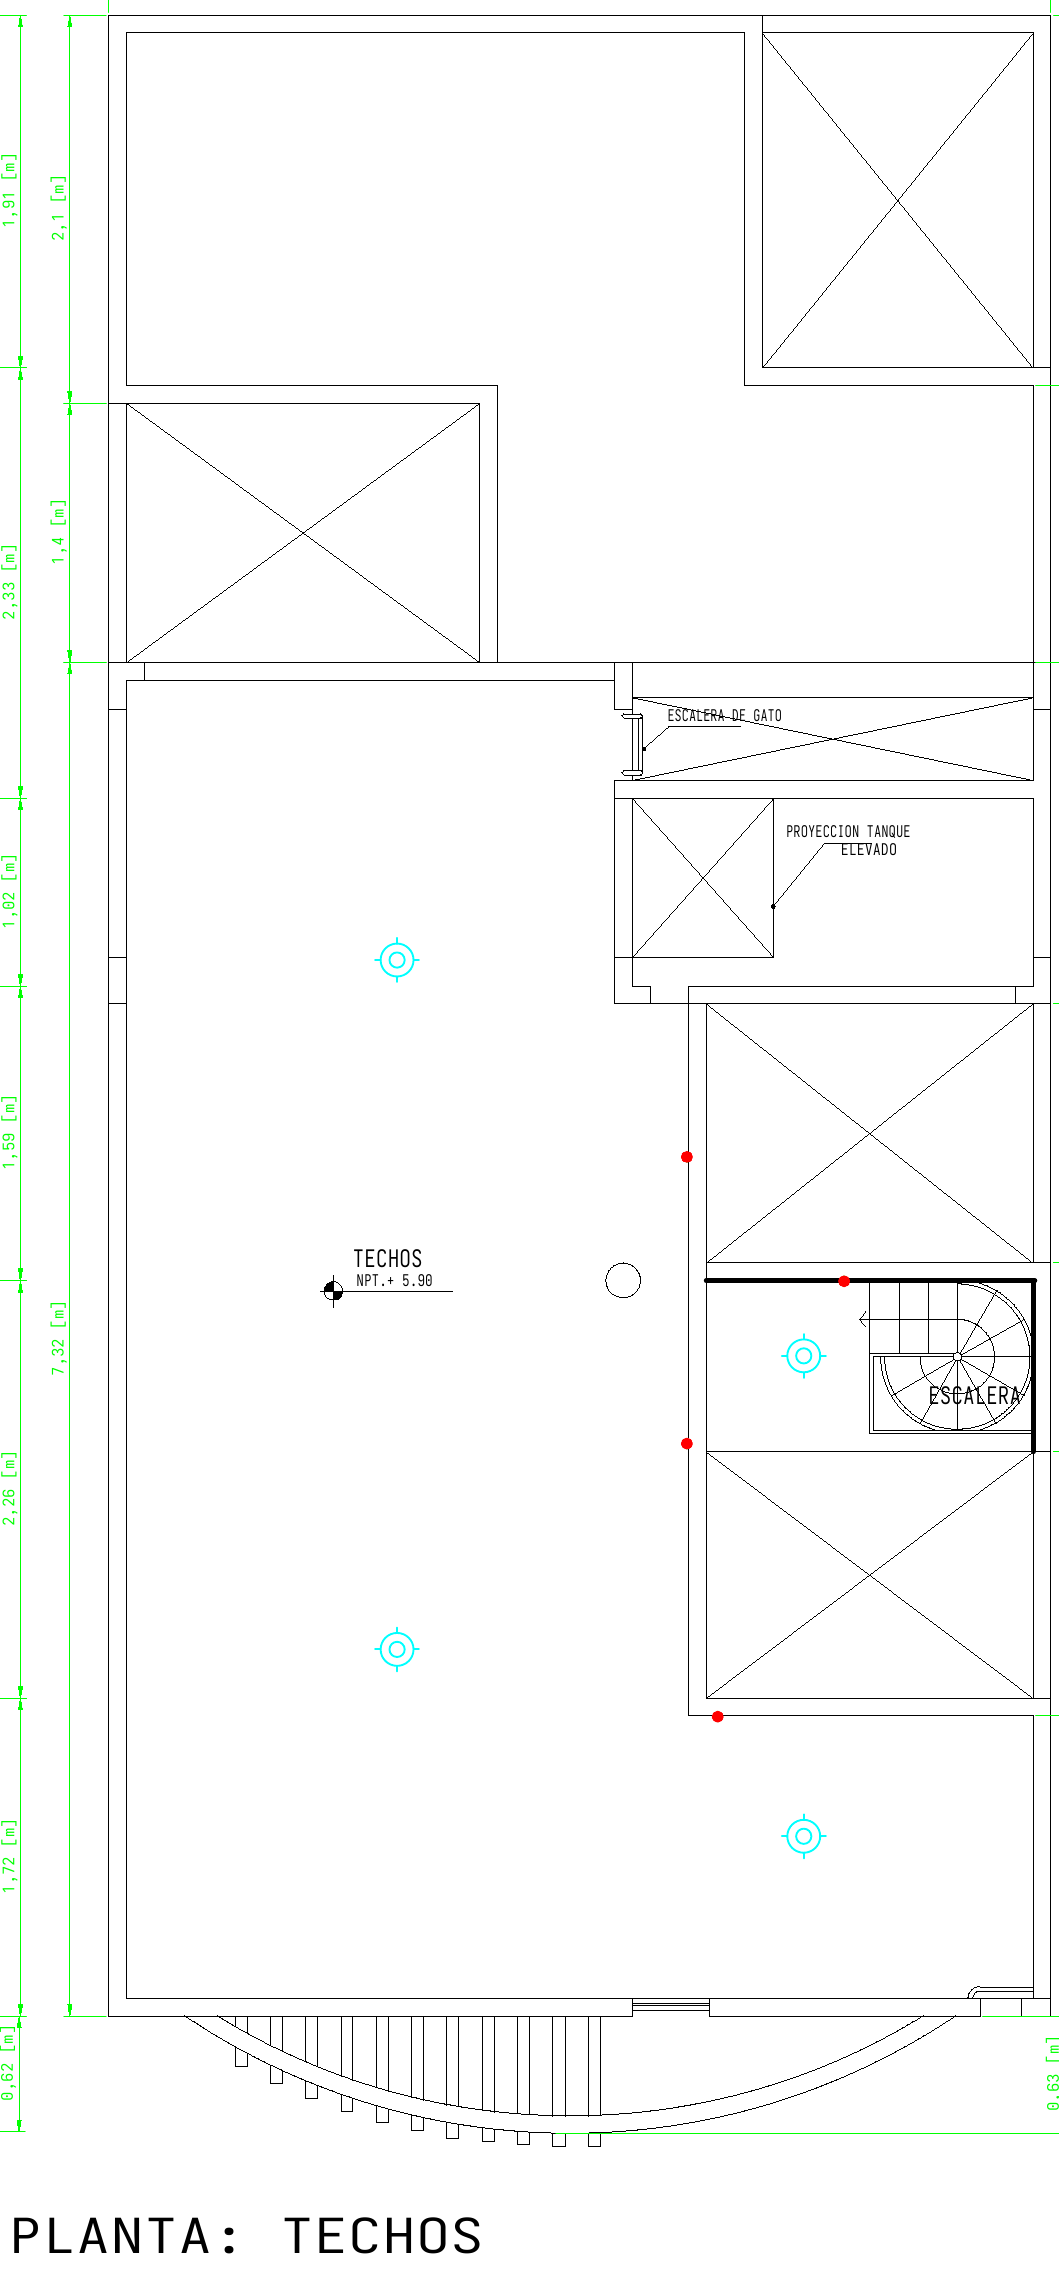
\includegraphics[width=0.85\linewidth]{images/PlanoArquitectonico-plantatechos.png}
\caption{Plano — Planta de techos (4 luminarias).}
\label{fig:plano_techos}
\end{figure}

\subsection{Cálculos eléctricos}

La resistencia de cada luminaria se deriva de su especificación nominal:
\begin{equation}
  R = \frac{V^2}{P} = \frac{120^2}{60} = 240~\Omega
  \label{eq:r_lamp}
\end{equation}

\subsubsection{Circuito global en paralelo — 44 luminarias}

\begin{align}
  R_{eq,p} &= \frac{240}{44} \approx 5{,}45~\Omega \\
  I_{total} &= \frac{120}{5{,}45} \approx 22{,}0~\text{A} \\
  I_k &= \frac{120}{240} = 0{,}5~\text{A}, \quad P_k = 60~\text{W} \\
  P_{total} &= 44 \times 60 = 2\,640~\text{W}
\end{align}
Con 5~h/día de uso: $E = 2{,}640 \times 5 = 13{,}2~\text{kWh/día}$.

\subsubsection{Circuito global en serie — 44 luminarias}

\begin{align}
  R_{eq,s} &= 44 \times 240 = 10\,560~\Omega \\
  I_{total} &= \frac{120}{10\,560} \approx 11{,}36~\text{mA} \\
  V_k &= \frac{120}{44} \approx 2{,}73~\text{V}, \quad P_k \approx 30{,}9~\text{mW} \\
  P_{total} &\approx 1{,}36~\text{W}
\end{align}

Con 44 elementos en cadena, cada lámpara recibe apenas el 2{,}3\% de la tensión nominal y disipa menos del 0{,}1\% de su potencia de diseño.

\textit{Nota:} Los valores de la Tabla~\ref{tab:sim_serie} corresponden al análisis \textit{por ambiente} (cada ambiente analizado como circuito independiente de $n_i$ lámparas). Los valores del circuito global —todas las 44 luminarias en una sola cadena— son los calculados arriba y validados en simulación.

%% ─── Simulación ─────────────────────────────────────────────────────────────
\section{Simulación y análisis de resultados}

\subsection{Principio de control: circuito con una lámpara}

Antes de escalar al proyecto completo, se implementó un circuito didáctico de una sola lámpara ($R = 240~\Omega$, $V_s = 120$~V) para comparar directamente el mando manual y el automático.

En el mando automático, un interruptor DIP-81 representa el detector de presencia: en verde simula persona detectada (señal activa) y en negro indica ausencia. Este interruptor controla la bobina de un relé; al energizarse, el contacto de potencia del relé cierra el circuito de la lámpara. La Figura~\ref{fig:manual_auto_apagado} muestra ambos circuitos apagados; la Figura~\ref{fig:manual_auto_encendido}, ambos encendidos.

\begin{figure}[H]
\centering
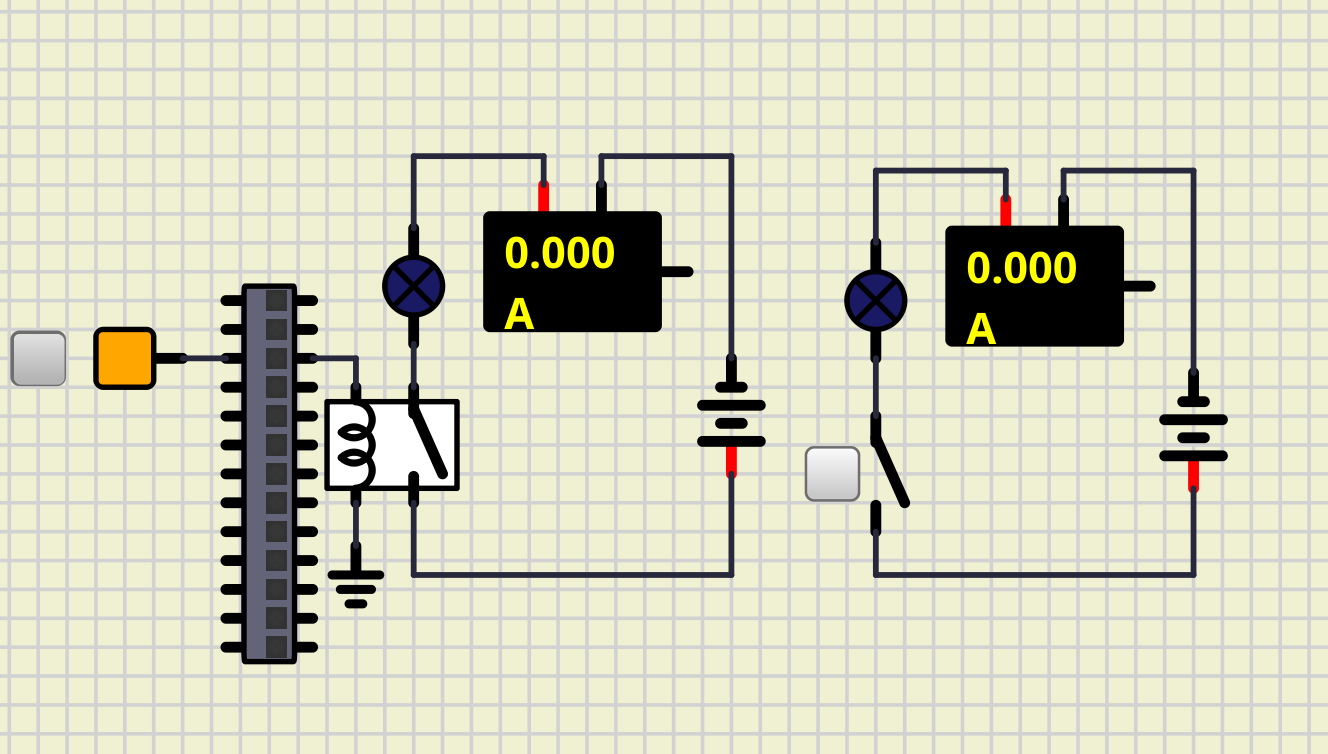
\includegraphics[width=0.85\linewidth]{images/circuito sensillo con interruptor manual e interruptor automatico apagados.png}
\caption{Circuito simple — mando manual (izq.) y automático (der.), estado apagado.}
\label{fig:manual_auto_apagado}
\end{figure}

\begin{figure}[H]
\centering
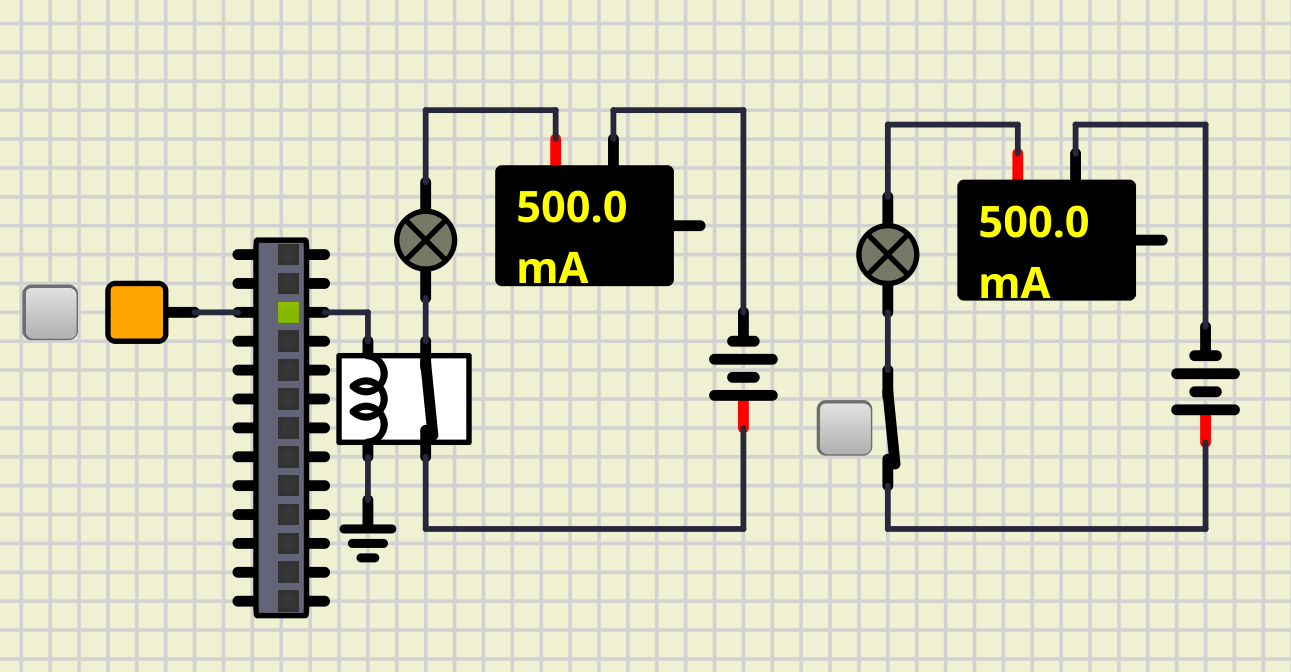
\includegraphics[width=0.85\linewidth]{images/circuito sensillo con interruptor manual e interruptor automatico encendidos.png}
\caption{Circuito simple — mando manual (izq.) y automático (der.), estado encendido.}
\label{fig:manual_auto_encendido}
\end{figure}

Este principio se escaló al proyecto completo sustituyendo el relé individual por relés de potencia por planta.

\subsection{Mando manual — circuito completo}

La Figura~\ref{fig:sig_ovalo} aclara la simbología de SimulIDE: el óvalo rojo indica nodo con tensión activa.

\begin{figure}[H]
\centering
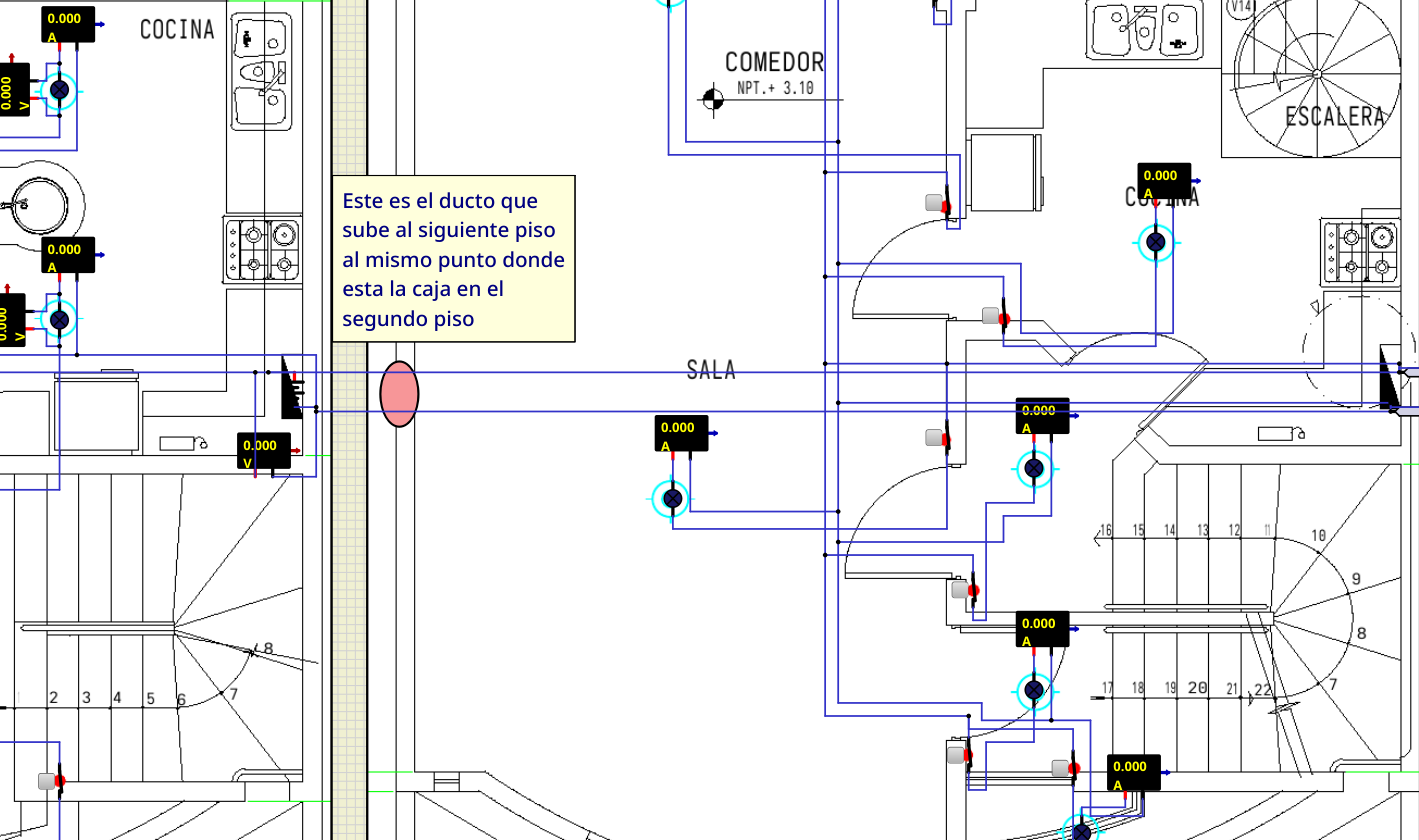
\includegraphics[width=0.85\linewidth]{images/significado del ovalo rojo.png}
\caption{Simbología SimulIDE: nodo de tensión activo (óvalo rojo).}
\label{fig:sig_ovalo}
\end{figure}

Las Figuras~\ref{fig:manual_sinsimu} y \ref{fig:manual_p1_sinsimu} muestran el circuito antes de energizar; las Figuras~\ref{fig:manual_encendido} y \ref{fig:manual_p1_encendido}, el estado con todas las luminarias activas.

\begin{figure}[H]
\centering
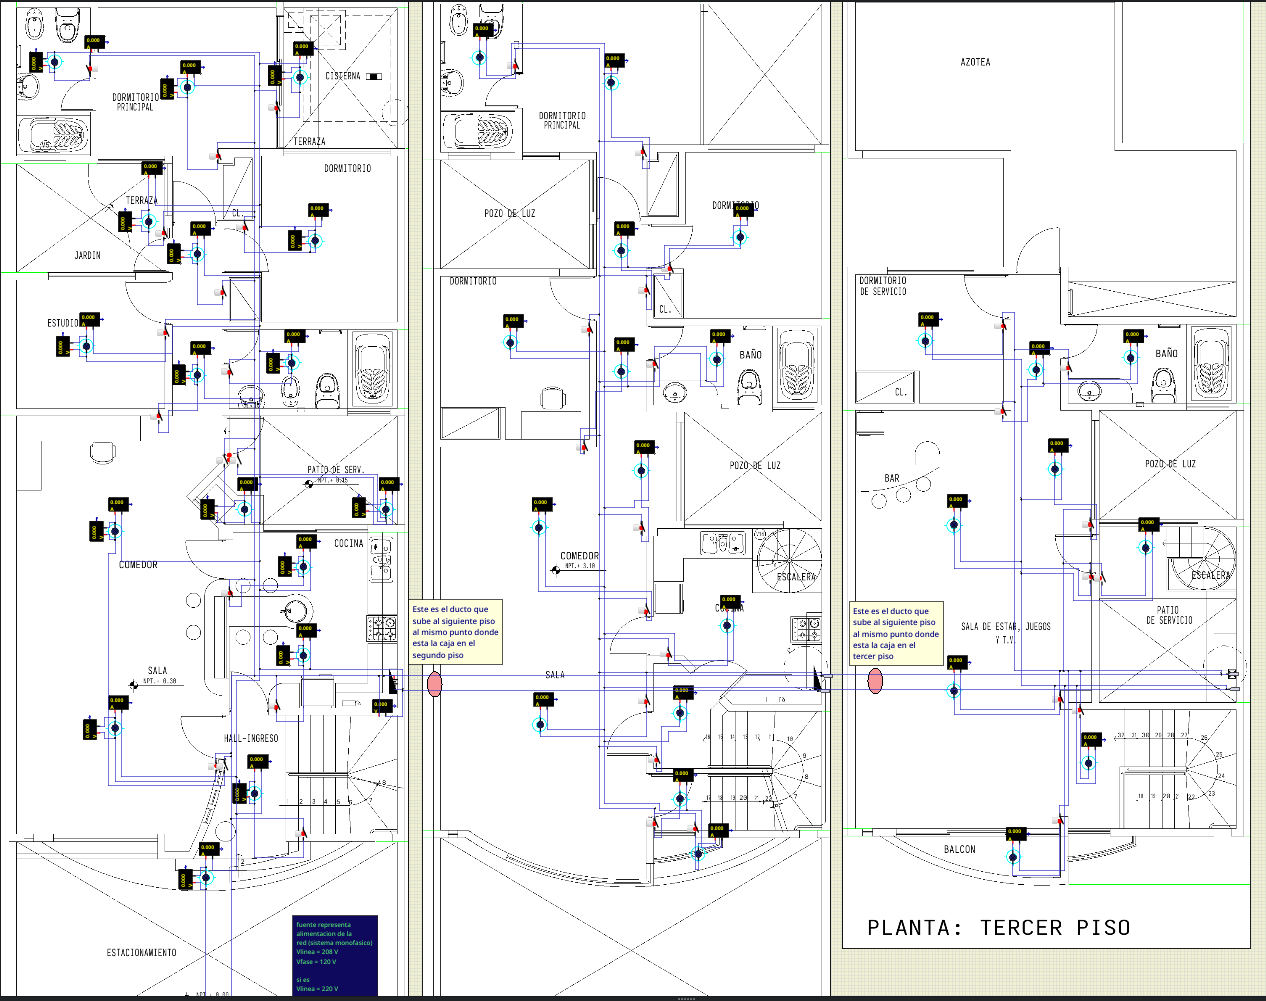
\includegraphics[width=0.85\linewidth]{images/manual sin simular todas las plantas.png}
\caption{Mando manual — cuatro plantas sin energizar.}
\label{fig:manual_sinsimu}
\end{figure}

\begin{figure}[H]
\centering
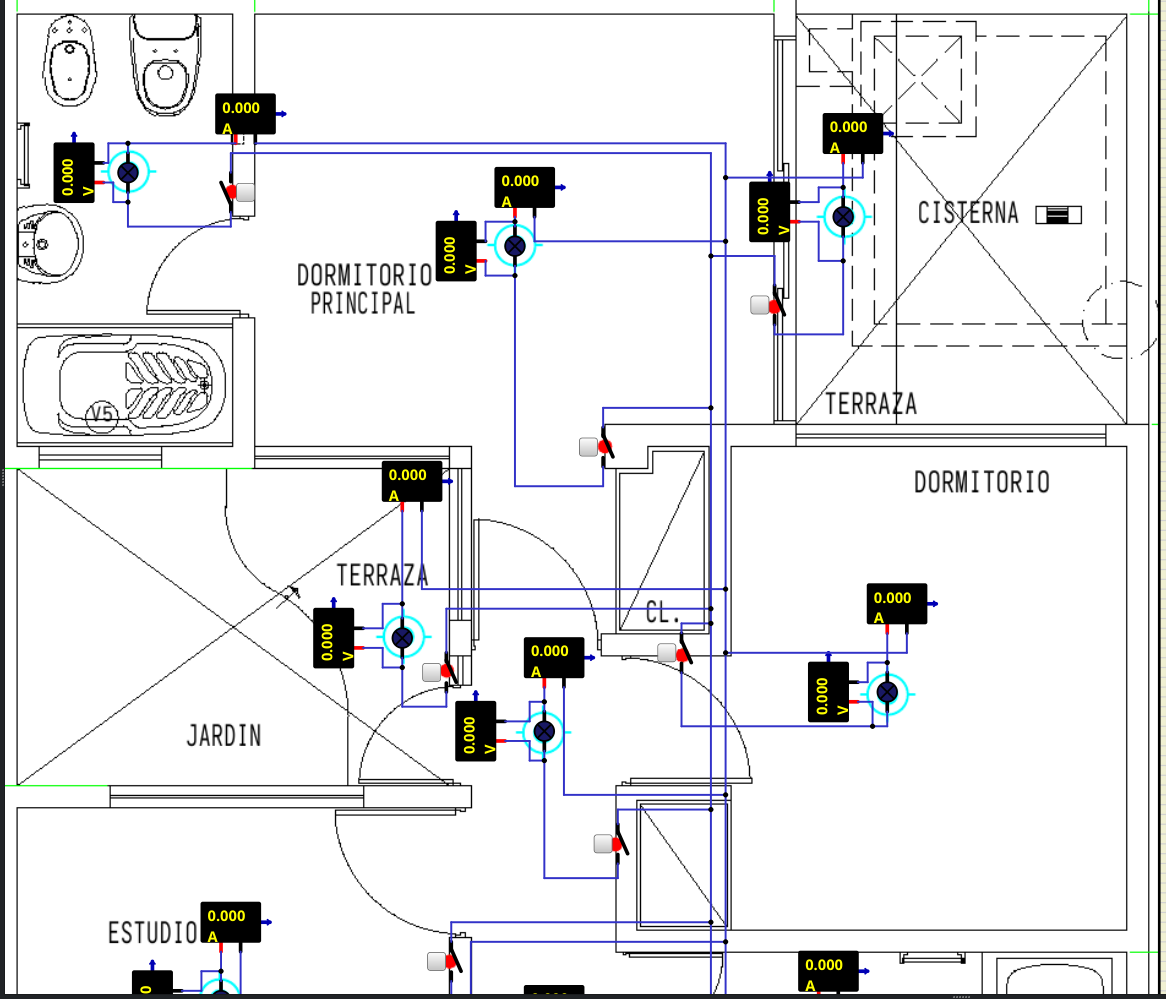
\includegraphics[width=0.85\linewidth]{images/manual sin simular planta 1_1 .png}
\caption{Mando manual — primer piso sin energizar (17 luminarias).}
\label{fig:manual_p1_sinsimu}
\end{figure}

\begin{figure}[H]
\centering
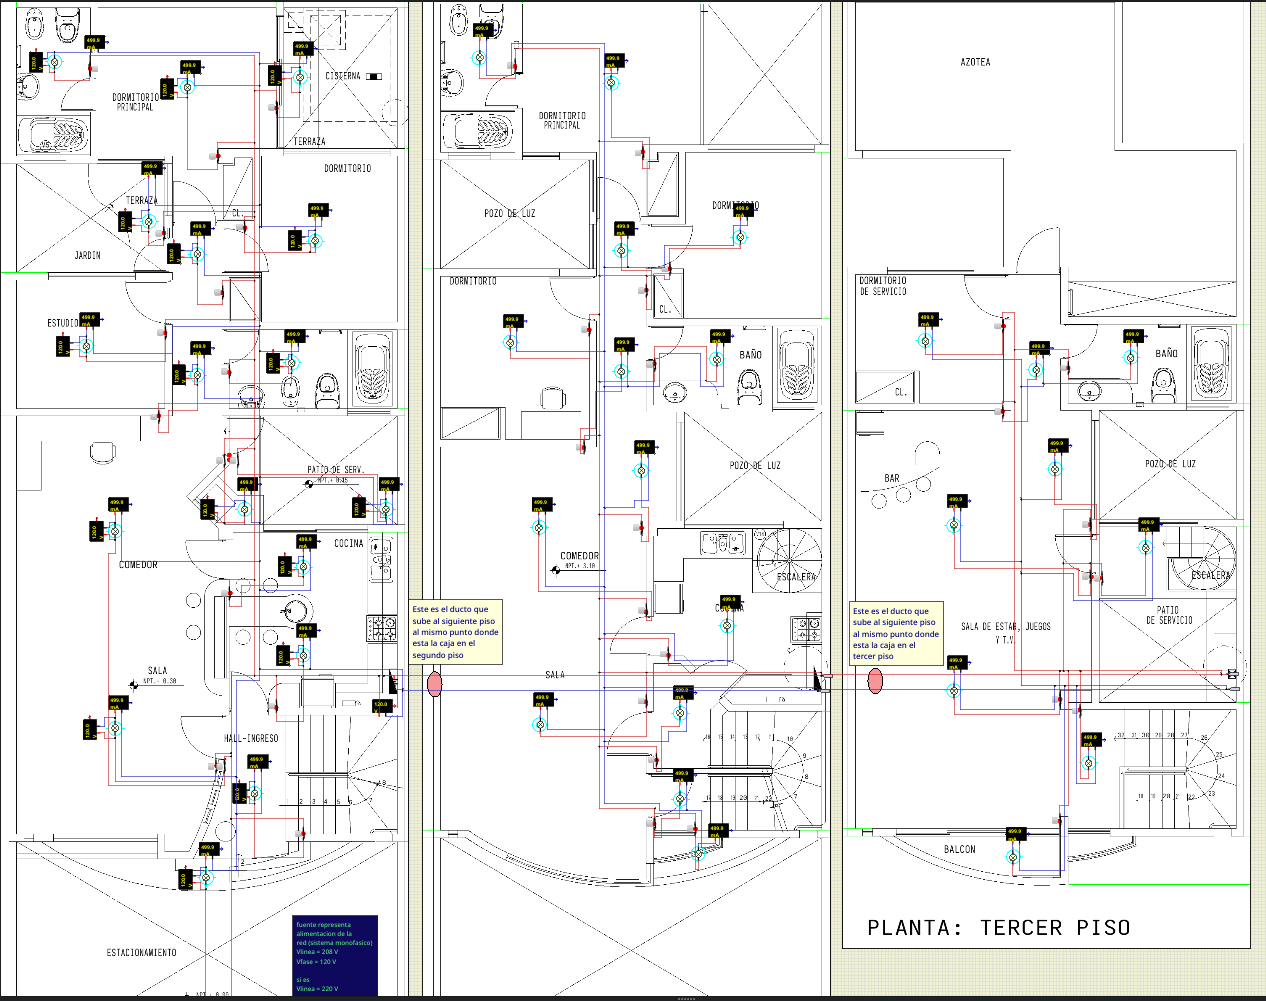
\includegraphics[width=0.85\linewidth]{images/mual simulado todas las plantas todos encendidos.png}
\caption{Mando manual simulado — 44 luminarias encendidas.}
\label{fig:manual_encendido}
\end{figure}

\begin{figure}[H]
\centering
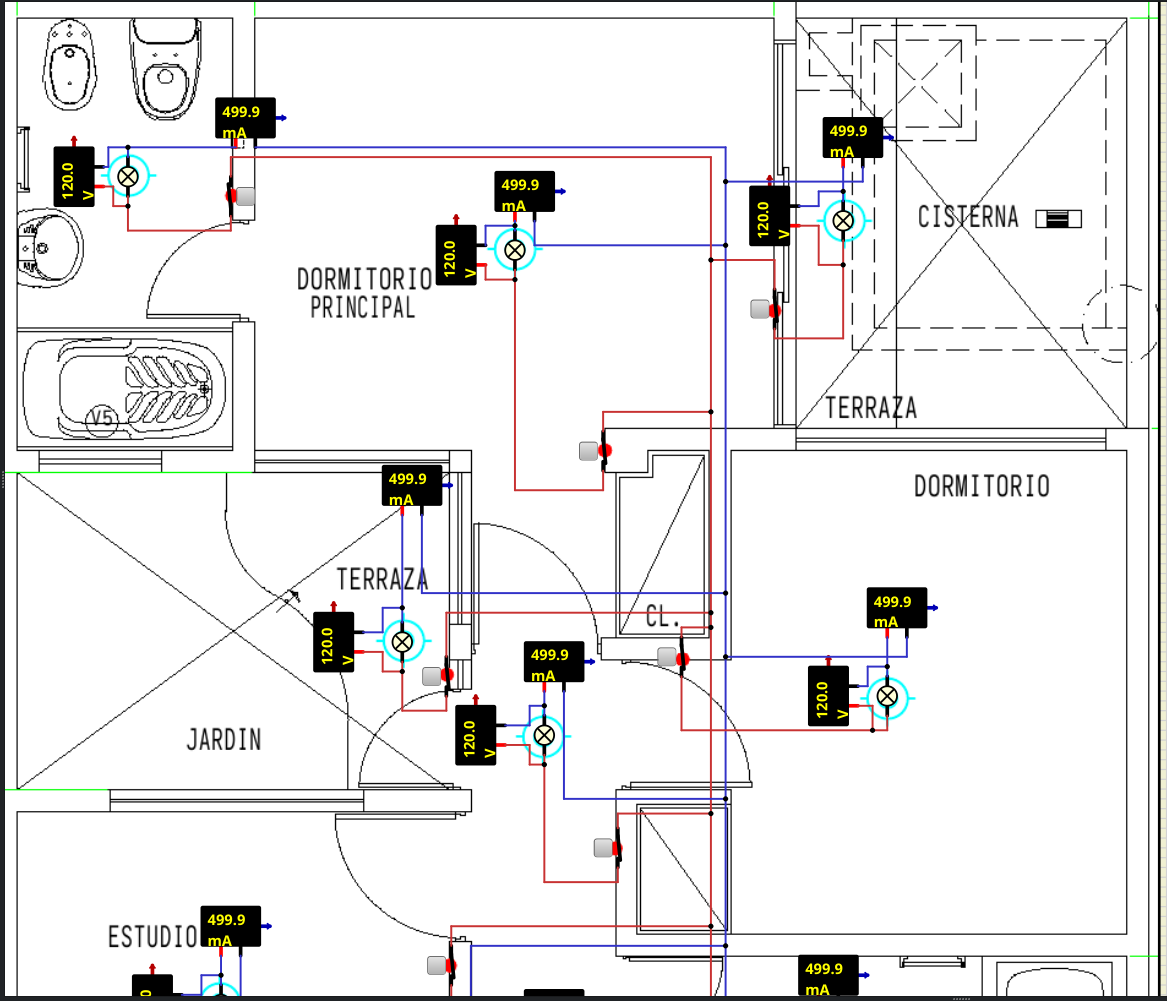
\includegraphics[width=0.85\linewidth]{images/mual simulado primera planta todos encendidos.png}
\caption{Mando manual simulado — primer piso en operación normal.}
\label{fig:manual_p1_encendido}
\end{figure}

\subsection{Mando automático — circuito completo}

El esquema automático escala el principio del circuito simple: un relé de potencia por planta, gobernado por detectores de presencia (DIP-81), reemplaza los interruptores manuales. Las Figuras~\ref{fig:auto_3plantas}--\ref{fig:auto_global} confirman que la lógica de mando centralizado opera correctamente sobre las 44 luminarias.

\begin{figure}[H]
\centering
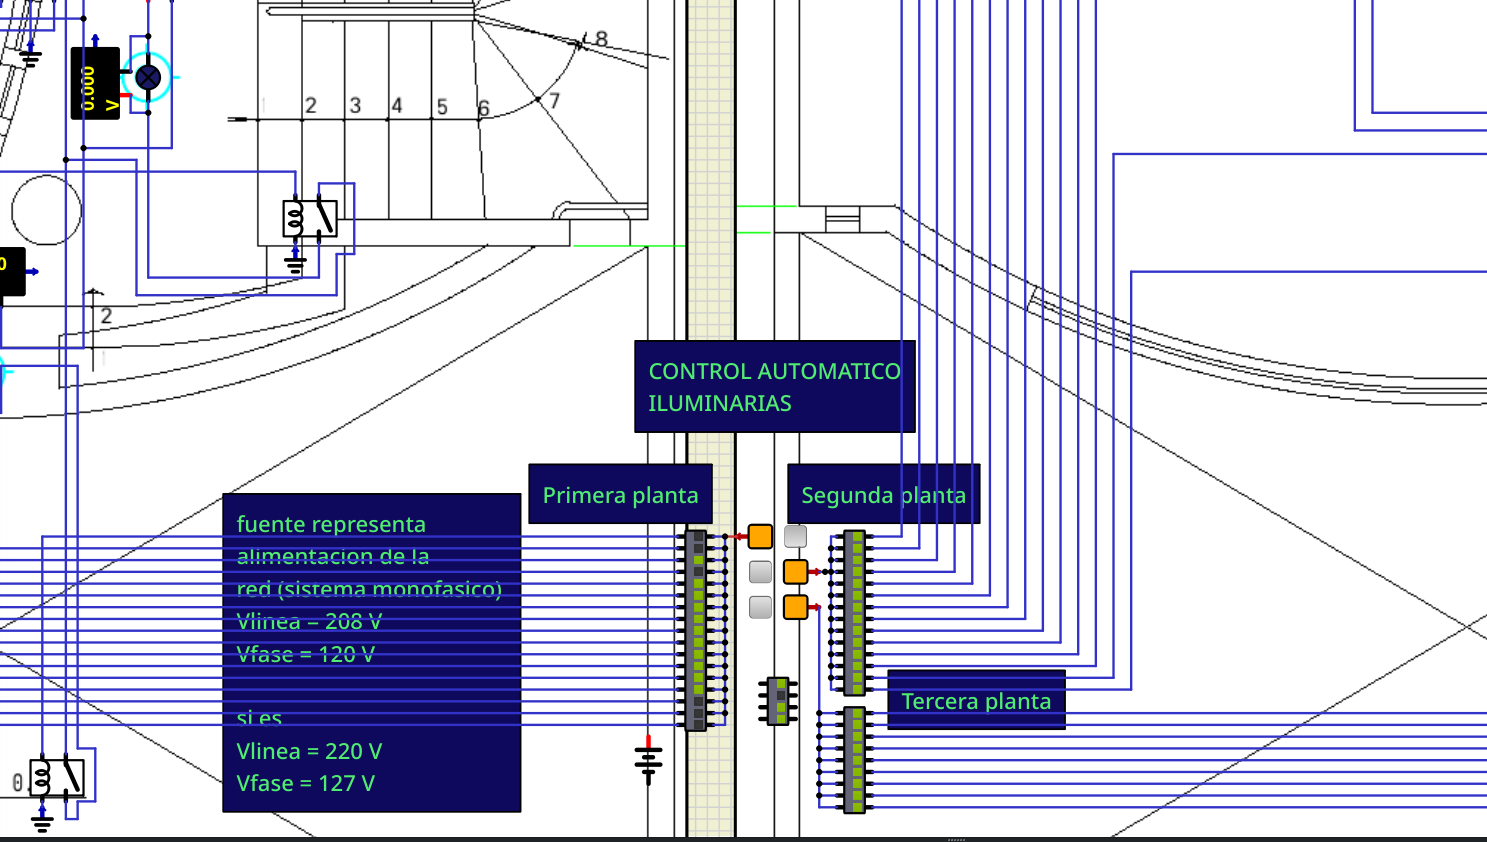
\includegraphics[width=0.85\linewidth]{images/control automatico 3 plantas.png}
\caption{Control automático — tres plantas habitables, relés activados.}
\label{fig:auto_3plantas}
\end{figure}

\begin{figure}[H]
\centering
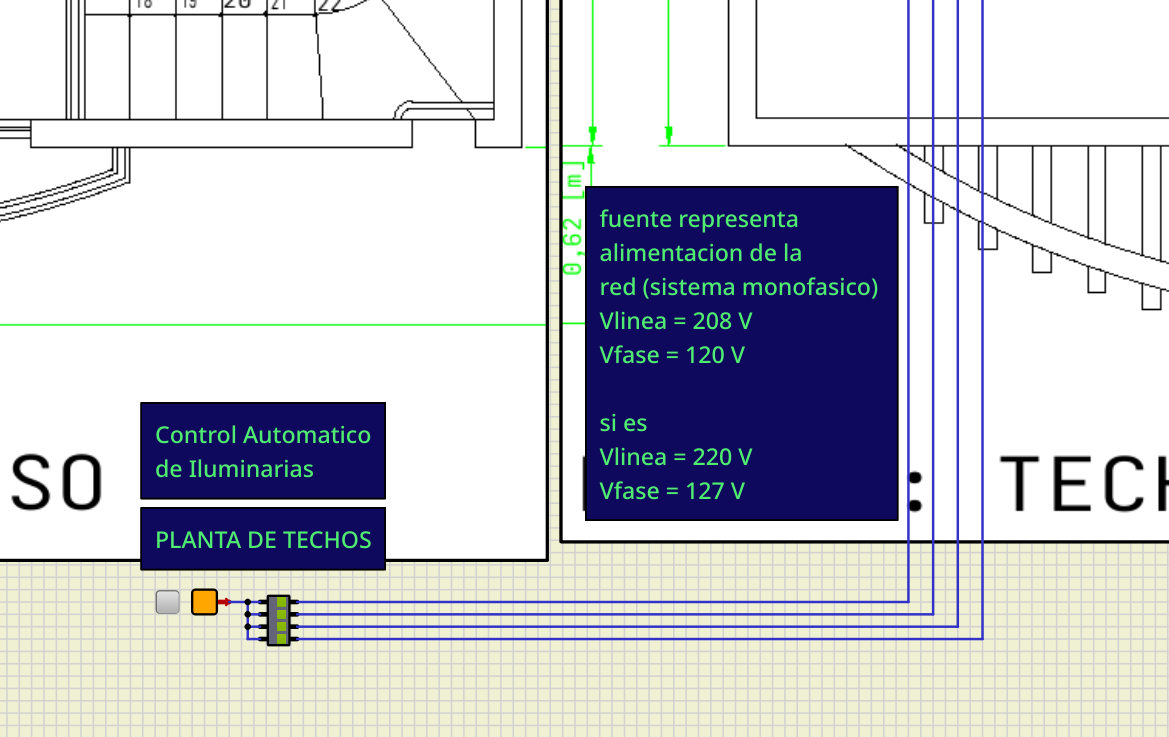
\includegraphics[width=0.85\linewidth]{images/control automatico planta de techos.png}
\caption{Control automático — planta de techos (4 luminarias).}
\label{fig:auto_techos}
\end{figure}

\begin{figure}[H]
\centering
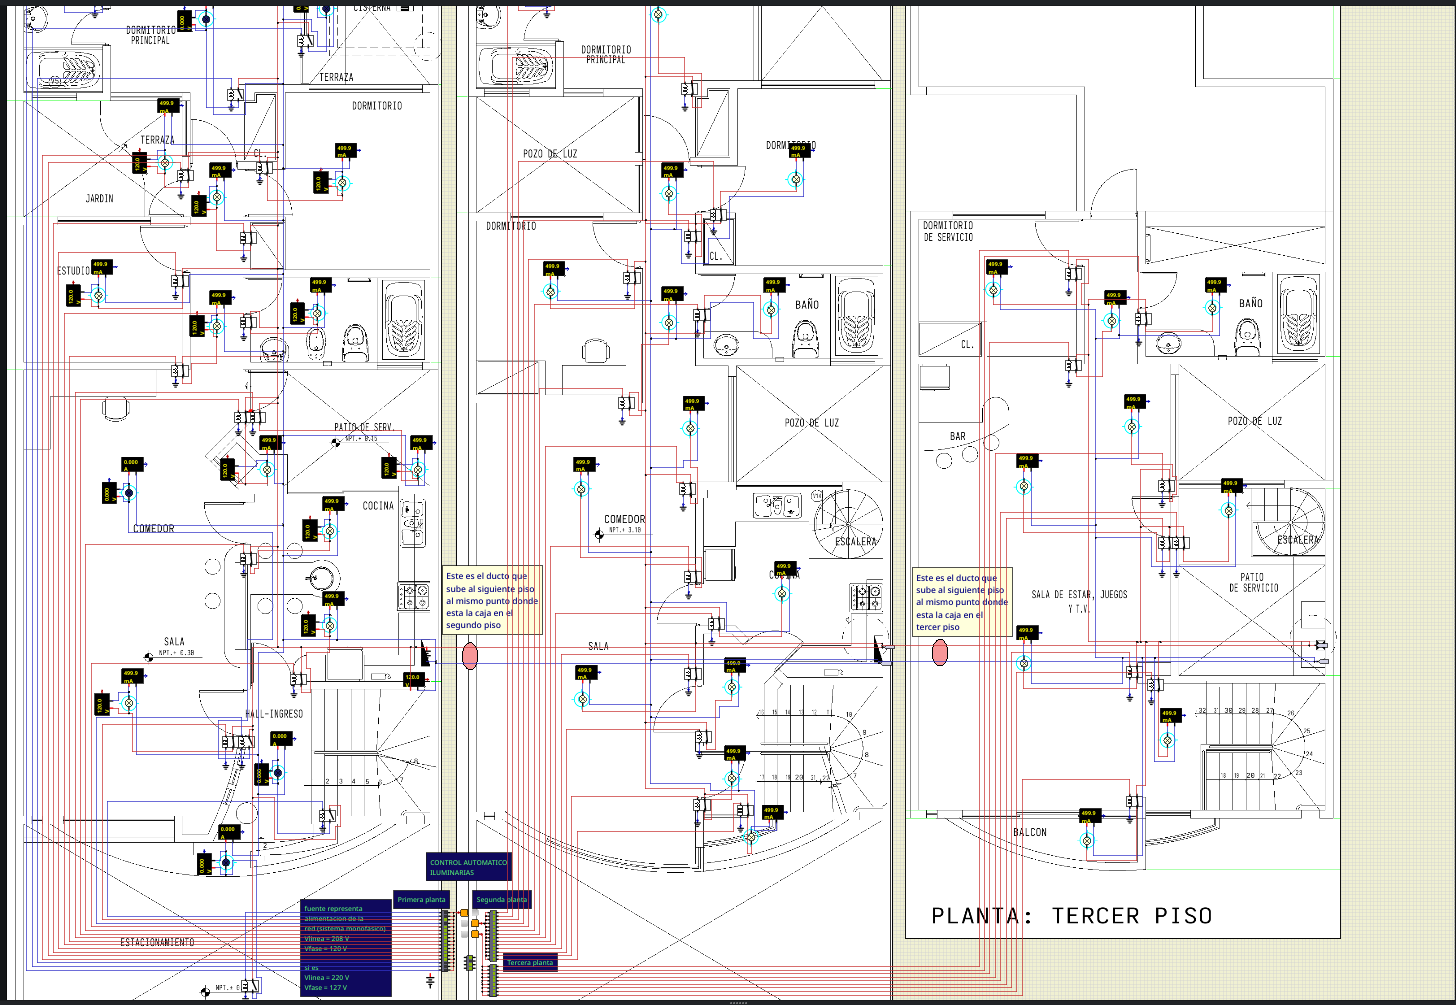
\includegraphics[width=0.85\linewidth]{images/automatico simulado todas las plantas todos encendidos.png}
\caption{Control automático simulado — 44 luminarias encendidas.}
\label{fig:auto_global}
\end{figure}

\subsection{Resultados de simulación — topología paralelo}

La Tabla~\ref{tab:sim_paralelo} presenta los resultados por ambiente en la topología paralelo. En todos los casos el simulador confirmó $V_k = 120$~V y $I_k = 0{,}5$~A por luminaria, independientemente del número de ramas activas, en perfecta concordancia con el modelo analítico.

\begin{table*}[H]
\centering
\caption{Simulación 1 — Circuito paralelo por ambiente ($V_s = 120$~V, $R = 240~\Omega$).}
\label{tab:sim_paralelo}
\begin{tabular}{llccccc}
\toprule
\textbf{Planta} & \textbf{Ambiente} & \textbf{$n$} & \textbf{$R_{eq}$ ($\Omega$)} & \textbf{$I_{tot}$ (A)} & \textbf{$V_k$ (V)} & \textbf{$P_{tot}$ (W)} \\
\midrule
\multirow{13}{*}{1.º Piso}
 & Estacionamiento        & 2 & 120{,}0 & 1{,}000 & 120 & 120{,}0 \\
 & Hall – Ingreso         & 1 & 240{,}0 & 0{,}500 & 120 &  60{,}0 \\
 & Sala                   & 2 & 120{,}0 & 1{,}000 & 120 & 120{,}0 \\
 & Comedor                & 2 & 120{,}0 & 1{,}000 & 120 & 120{,}0 \\
 & Cocina                 & 1 & 240{,}0 & 0{,}500 & 120 &  60{,}0 \\
 & Patio de Servicio      & 1 & 240{,}0 & 0{,}500 & 120 &  60{,}0 \\
 & Dormitorio Principal   & 2 & 120{,}0 & 1{,}000 & 120 & 120{,}0 \\
 & Baño                   & 1 & 240{,}0 & 0{,}500 & 120 &  60{,}0 \\
 & Dormitorio             & 1 & 240{,}0 & 0{,}500 & 120 &  60{,}0 \\
 & Estudio                & 1 & 240{,}0 & 0{,}500 & 120 &  60{,}0 \\
 & Terraza                & 1 & 240{,}0 & 0{,}500 & 120 &  60{,}0 \\
 & Jardín                 & 1 & 240{,}0 & 0{,}500 & 120 &  60{,}0 \\
 & Cisterna / Terraza ext & 1 & 240{,}0 & 0{,}500 & 120 &  60{,}0 \\
\midrule
\multirow{8}{*}{2.º Piso}
 & Dormitorio Principal   & 2 & 120{,}0 & 1{,}000 & 120 & 120{,}0 \\
 & Dormitorio             & 2 & 120{,}0 & 1{,}000 & 120 & 120{,}0 \\
 & Baño                   & 1 & 240{,}0 & 0{,}500 & 120 &  60{,}0 \\
 & Sala                   & 2 & 120{,}0 & 1{,}000 & 120 & 120{,}0 \\
 & Comedor                & 2 & 120{,}0 & 1{,}000 & 120 & 120{,}0 \\
 & Cocina                 & 2 & 120{,}0 & 1{,}000 & 120 & 120{,}0 \\
 & Escalera               & 1 & 240{,}0 & 0{,}500 & 120 &  60{,}0 \\
 & Pozo de Luz            & 2 & 120{,}0 & 1{,}000 & 120 & 120{,}0 \\
\midrule
\multirow{9}{*}{3.er Piso}
 & Sala Estar / TV        & 2 & 120{,}0 & 1{,}000 & 120 & 120{,}0 \\
 & Bar                    & 1 & 240{,}0 & 0{,}500 & 120 &  60{,}0 \\
 & Dorm. de Servicio      & 1 & 240{,}0 & 0{,}500 & 120 &  60{,}0 \\
 & Baño                   & 1 & 240{,}0 & 0{,}500 & 120 &  60{,}0 \\
 & Azotea                 & 1 & 240{,}0 & 0{,}500 & 120 &  60{,}0 \\
 & Patio de Servicio      & 1 & 240{,}0 & 0{,}500 & 120 &  60{,}0 \\
 & Pozo de Luz            & 1 & 240{,}0 & 0{,}500 & 120 &  60{,}0 \\
 & Balcón                 & 1 & 240{,}0 & 0{,}500 & 120 &  60{,}0 \\
 & Escalera               & 0 &    —    &    —    &  —  &     —   \\
\midrule
\multirow{3}{*}{Techos}
 & Área cubierta          & 2 & 120{,}0 & 1{,}000 & 120 & 120{,}0 \\
 & Proy. Tanque           & 1 & 240{,}0 & 0{,}500 & 120 &  60{,}0 \\
 & Escalera de Gato       & 1 & 240{,}0 & 0{,}500 & 120 &  60{,}0 \\
\midrule
\textbf{Global (44 lum.)} & & \textbf{44} & \textbf{5{,}45} & \textbf{22{,}0} & \textbf{120} & \textbf{2\,640} \\
\bottomrule
\end{tabular}
\end{table*}

\subsection{Resultados de simulación — topología serie}

La Tabla~\ref{tab:sim_serie} presenta los valores por ambiente en configuración serie. Se observa que los ambientes con una sola luminaria no presentan división de tensión ($V_k = 120$~V en ese análisis independiente), mientras que los ambientes con dos lámparas en cadena reciben 60~V por elemento. El dato crítico es el circuito \textit{global}: con las 44 luminarias en una única cadena, SimulIDE confirmó $V_k = 2{,}73$~V e $I = 11{,}36$~mA, en acuerdo exacto con el cálculo analítico.

\begin{table*}[H]
\centering
\caption{Simulación 2 — Circuito serie por ambiente ($V_s = 120$~V, $R = 240~\Omega$).}
\label{tab:sim_serie}
\begin{tabular}{llccccc}
\toprule
\textbf{Planta} & \textbf{Ambiente} & \textbf{$n$} & \textbf{$R_{eq}$ ($\Omega$)} & \textbf{$I_{tot}$ (A)} & \textbf{$V_k$ (V)} & \textbf{$P_{tot}$ (W)} \\
\midrule
\multirow{13}{*}{1.º Piso}
 & Estacionamiento        & 2 &  480 & 0{,}250 &  60{,}0 & 30{,}0 \\
 & Hall – Ingreso         & 1 &  240 & 0{,}500 & 120{,}0 & 60{,}0 \\
 & Sala                   & 2 &  480 & 0{,}250 &  60{,}0 & 30{,}0 \\
 & Comedor                & 2 &  480 & 0{,}250 &  60{,}0 & 30{,}0 \\
 & Cocina                 & 1 &  240 & 0{,}500 & 120{,}0 & 60{,}0 \\
 & Patio de Servicio      & 1 &  240 & 0{,}500 & 120{,}0 & 60{,}0 \\
 & Dormitorio Principal   & 2 &  480 & 0{,}250 &  60{,}0 & 30{,}0 \\
 & Baño                   & 1 &  240 & 0{,}500 & 120{,}0 & 60{,}0 \\
 & Dormitorio             & 1 &  240 & 0{,}500 & 120{,}0 & 60{,}0 \\
 & Estudio                & 1 &  240 & 0{,}500 & 120{,}0 & 60{,}0 \\
 & Terraza                & 1 &  240 & 0{,}500 & 120{,}0 & 60{,}0 \\
 & Jardín                 & 1 &  240 & 0{,}500 & 120{,}0 & 60{,}0 \\
 & Cisterna / Terraza ext & 1 &  240 & 0{,}500 & 120{,}0 & 60{,}0 \\
\midrule
\multirow{8}{*}{2.º Piso}
 & Dormitorio Principal   & 2 &  480 & 0{,}250 &  60{,}0 & 30{,}0 \\
 & Dormitorio             & 2 &  480 & 0{,}250 &  60{,}0 & 30{,}0 \\
 & Baño                   & 1 &  240 & 0{,}500 & 120{,}0 & 60{,}0 \\
 & Sala                   & 2 &  480 & 0{,}250 &  60{,}0 & 30{,}0 \\
 & Comedor                & 2 &  480 & 0{,}250 &  60{,}0 & 30{,}0 \\
 & Cocina                 & 2 &  480 & 0{,}250 &  60{,}0 & 30{,}0 \\
 & Escalera               & 1 &  240 & 0{,}500 & 120{,}0 & 60{,}0 \\
 & Pozo de Luz            & 2 &  480 & 0{,}250 &  60{,}0 & 30{,}0 \\
\midrule
\multirow{9}{*}{3.er Piso}
 & Sala Estar / TV        & 2 &  480 & 0{,}250 &  60{,}0 & 30{,}0 \\
 & Bar                    & 1 &  240 & 0{,}500 & 120{,}0 & 60{,}0 \\
 & Dorm. de Servicio      & 1 &  240 & 0{,}500 & 120{,}0 & 60{,}0 \\
 & Baño                   & 1 &  240 & 0{,}500 & 120{,}0 & 60{,}0 \\
 & Azotea                 & 1 &  240 & 0{,}500 & 120{,}0 & 60{,}0 \\
 & Patio de Servicio      & 1 &  240 & 0{,}500 & 120{,}0 & 60{,}0 \\
 & Pozo de Luz            & 1 &  240 & 0{,}500 & 120{,}0 & 60{,}0 \\
 & Balcón                 & 1 &  240 & 0{,}500 & 120{,}0 & 60{,}0 \\
 & Escalera               & 0 &   —  &    —    &     —   &    —   \\
\midrule
\multirow{3}{*}{Techos}
 & Área cubierta          & 2 &  480 & 0{,}250 &  60{,}0 & 30{,}0 \\
 & Proy. Tanque           & 1 &  240 & 0{,}500 & 120{,}0 & 60{,}0 \\
 & Escalera de Gato       & 1 &  240 & 0{,}500 & 120{,}0 & 60{,}0 \\
\midrule
\textbf{Global (44 lum.)} & & \textbf{44} & \textbf{10\,560} & \textbf{0{,}011} & \textbf{2{,}73} & \textbf{1{,}36} \\
\bottomrule
\end{tabular}
\end{table*}

\subsection{Contraste analítico vs.\ simulación}

La Tabla~\ref{tab:contraste} compara los valores globales calculados analíticamente con los registrados en SimulIDE para el circuito completo de 44 luminarias.

\begin{table}[H]
\centering
\caption{Contraste analítico vs.\ simulación — circuito global de 44 luminarias.}
\label{tab:contraste}
\begin{tabular}{lccc}
\toprule
\textbf{Magnitud} & \textbf{Analítico} & \textbf{SimulIDE} & \textbf{Error} \\
\midrule
\multicolumn{4}{l}{\textit{Paralelo}} \\
$R_{eq}$ ($\Omega$)    & 5{,}45   & 5{,}45   & 0\% \\
$I_{total}$ (A)        & 22{,}00  & 22{,}00  & 0\% \\
$V_k$ (V)              & 120{,}0  & 120{,}0  & 0\% \\
$P_{total}$ (W)        & 2\,640   & 2\,640   & 0\% \\
\midrule
\multicolumn{4}{l}{\textit{Serie}} \\
$R_{eq}$ ($\Omega$)    & 10\,560  & 10\,560  & 0\% \\
$I_{total}$ (mA)       & 11{,}36  & 11{,}36  & 0\% \\
$V_k$ (V)              & 2{,}73   & 2{,}73   & 0\% \\
$P_{total}$ (W)        & 1{,}36   & 1{,}36   & 0\% \\
\bottomrule
\end{tabular}
\end{table}

La concordancia es total, lo que valida tanto el modelo como la implementación en SimulIDE. El error nulo se explica porque el simulador resuelve el mismo sistema de ecuaciones lineales que el modelo analítico, sin efectos no lineales ni parásitos.

\subsection{Comparativa de topologías}

La Tabla~\ref{tab:comparativa} sintetiza los aspectos técnicos diferenciadores.

\begin{table}[H]
\centering
\caption{Comparativa técnica — serie vs.\ paralelo.}
\label{tab:comparativa}
\begin{tabular}{lcc}
\toprule
\textbf{Aspecto} & \textbf{Serie} & \textbf{Paralelo} \\
\midrule
$V_k$ (V)                & 2{,}73 (2{,}3\%) & 120 (100\%)  \\
$I_{total}$              & 11{,}36 mA       & 22{,}0 A     \\
$P_k$                    & 30{,}9 mW        & 60 W         \\
$P_{total}$              & 1{,}36 W         & 2\,640 W     \\
Fallo unitario           & Apagado total    & Sin efecto   \\
Independencia de ramas   & No               & Sí           \\
Cumple RETIE             & No               & Sí           \\
Aplicación              & Experimental     & Residencial  \\
\bottomrule
\end{tabular}
\end{table}

El control automático no modifica las variables eléctricas del circuito de potencia: tensión y corriente en las cargas son idénticas a las del mando manual cuando el relé está activado. Su ventaja radica en desacoplar físicamente al operador del circuito de fuerza, lo que mejora la seguridad y el confort en instalaciones de varios niveles.

%% ─── Materiales ─────────────────────────────────────────────────────────────
\section{Lista de materiales}

\begin{itemize}
  \item 44 lámparas incandescentes 60~W / 120~V ($R = 240~\Omega$).
  \item Interruptores unipolares 10~A / 250~V, uno por planta (mando manual).
  \item Relés de bobina 12~V, uno por planta (mando automático).
  \item Conductor Cu \#12~AWG para ramal paralelo (22~A); \#14~AWG admisible solo en ramal serie.
  \item Fuente 120~V~CD para banco de pruebas.
  \item Software SimulIDE y AutoCAD.
  \item Cinta métrica, nivel y cámara fotográfica.
\end{itemize}

%% ─── Elementos seleccionados ────────────────────────────────────────────────
\section{Elementos seleccionados para el montaje real}

Con base en los resultados del análisis eléctrico —topología paralelo, corriente total de 22~A repartida en 44 luminarias— se seleccionaron los componentes físicos que conformarían la instalación real de la vivienda. Todos los elementos corresponden a la línea disponible en el mercado local colombiano y cumplen con las especificaciones mínimas exigidas por el RETIE y la NTC~2050.

\subsection{Luminaria}

Se seleccionó la \textbf{lámpara circular negra de 60~W, 5000~K, 120~V / 50--60~Hz, Ø900~mm~×~80~mm} (Figura~\ref{fig:lampara}). La temperatura de color de 5000~K corresponde a luz blanca fría, adecuada para zonas de trabajo (cocina, estudio, estacionamiento) y aceptable en zonas sociales. A 120~V y con $R = 240~\Omega$, la corriente de operación es 0{,}5~A y la potencia disipada es exactamente 60~W, coincidiendo con el modelo de simulación.

\begin{figure}[H]
\centering
\includegraphics[width=0.65\linewidth]{images/LAMPARA CIRCULAR\string\nNEGRA 60W 5000K\string\n120V 50-60HZ\string\nO900X80MM INC.png}
\caption{Lámpara circular 60~W / 5000~K / 120~V seleccionada para el proyecto.}
\label{fig:lampara}
\end{figure}

\subsection{Interruptor sencillo}

Para el mando manual se seleccionó un \textbf{interruptor sencillo unipolar} (Figura~\ref{fig:int_ficha}), cuya ficha técnica especifica operación a 120~V~CA / 10~A, contacto de plata de alta durabilidad y caja de montaje en pared de 2~×~4 pulgadas. Este dispositivo es el elemento de maniobra estándar en instalaciones residenciales colombianas y es compatible con los circuitos ramales dimensionados para 20~A cuando se usa como interruptor de control (no de protección).

\begin{figure}[H]
\centering
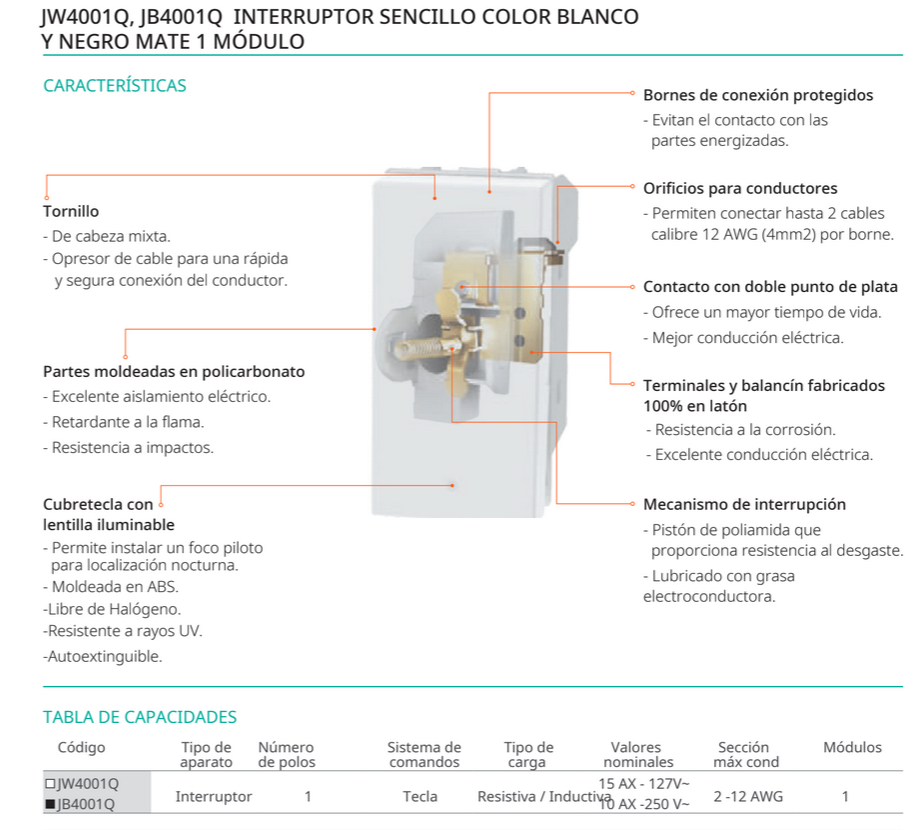
\includegraphics[width=0.75\linewidth]{images/ficha tecnica interruptor sencillo.png}
\caption{Ficha técnica del interruptor sencillo seleccionado.}
\label{fig:int_ficha}
\end{figure}

Las Figuras~\ref{fig:int_conexion} y \ref{fig:int_montaje} presentan, respectivamente, el diagrama de conexión eléctrica y el diagrama de montaje físico del interruptor en la caja de pared.

\begin{figure}[H]
\centering
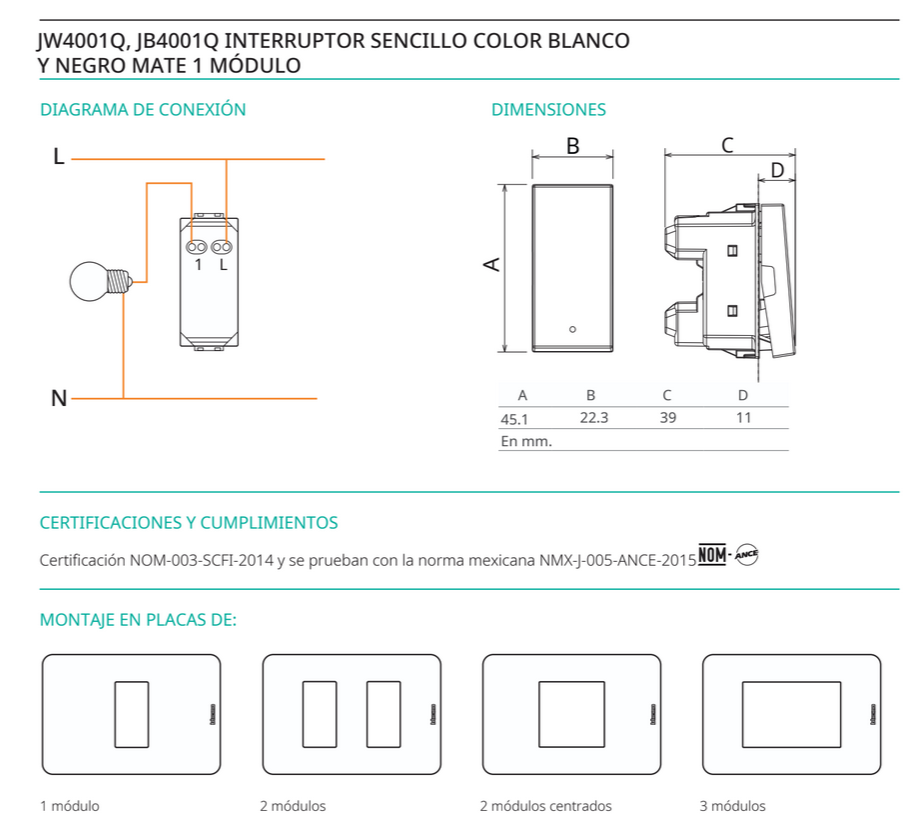
\includegraphics[width=0.75\linewidth]{images/diagrama de conexion del interruptor sencillo.png}
\caption{Diagrama de conexión del interruptor sencillo (fase — interruptor — luminaria — neutro).}
\label{fig:int_conexion}
\end{figure}

\begin{figure}[H]
\centering
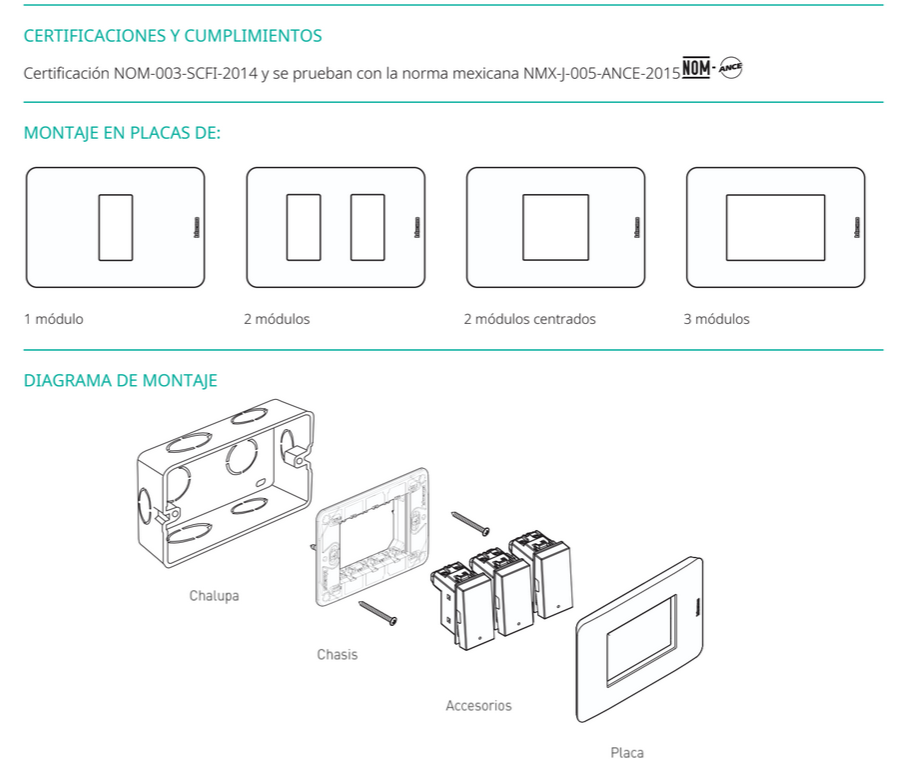
\includegraphics[width=0.75\linewidth]{images/diagrama de montaje del interruptor sencillo.png}
\caption{Diagrama de montaje del interruptor sencillo en caja de 2~×~4''.}
\label{fig:int_montaje}
\end{figure}

\subsection{Conductor}

Se especificó \textbf{cable THHN \#12~AWG sólido} (Figura~\ref{fig:cable}), con capacidad de conducción de 20~A en instalación en conduit, aislamiento termoplástico de 90~°C (THHN) resistente a la humedad y temperatura, conforme a NTC~2050 tabla 310-16. Este calibre es el mínimo requerido para los circuitos ramales del sistema en paralelo, dado que la corriente total de 22~A se sectoriza en ramales individuales de máximo 20~A. Para los ramales de planta de techos (4 luminarias, 2~A de demanda) sería técnicamente admisible \#14~AWG, pero se unifica en \#12~AWG para simplificar el inventario de materiales y agregar margen de seguridad.

\begin{figure}[H]
\centering
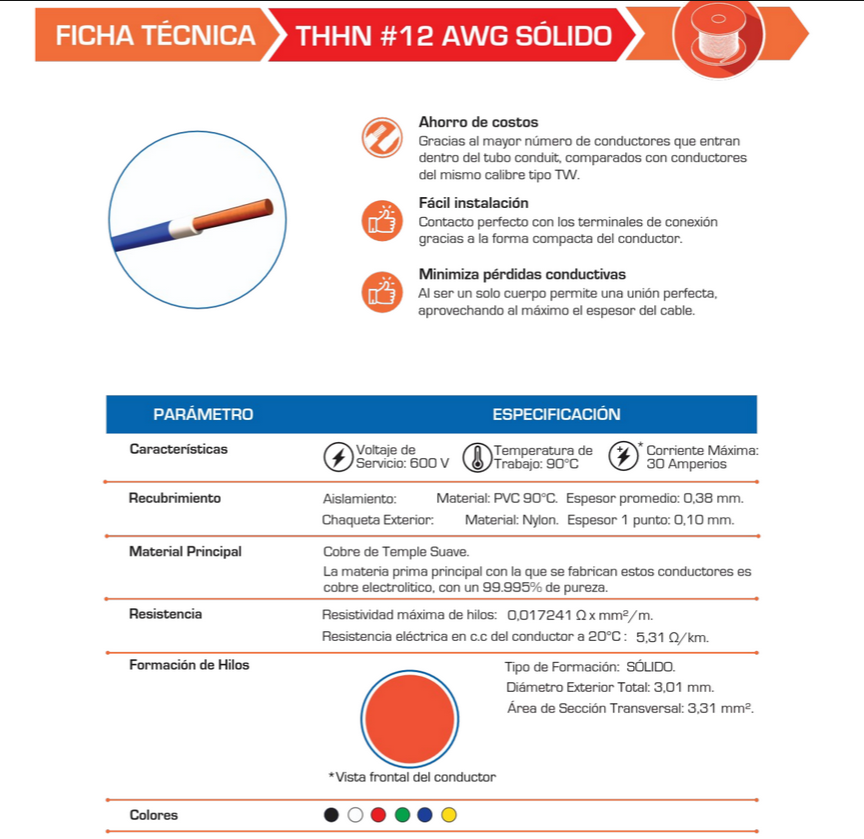
\includegraphics[width=0.85\linewidth]{images/ficha tecnica calibre THHN 12 AWG solido.png}
\caption{Ficha técnica del conductor THHN \#12~AWG sólido.}
\label{fig:cable}
\end{figure}

\subsection{Protección termomagnética}

Para la protección de cada ramal se seleccionó el \textbf{interruptor termomagnético de 25~A} de la línea disponible (Figura~\ref{fig:termo}). Aunque los ramales se dimensionaron para 20~A, el breaker de 25~A es el inmediatamente superior disponible en la referencia comercial consultada y opera dentro del margen permitido por la NTC~2050 para conductores \#12~AWG (capacidad 20~A), siempre que la carga real no supere dicho valor. En la práctica, cada ramal de iluminación demanda entre 1 y 8{,}5~A según el número de luminarias conectadas, por lo que el dispositivo de 25~A nunca opera cerca de su umbral térmico y ofrece protección adecuada contra cortocircuito.

\begin{figure}[H]
\centering
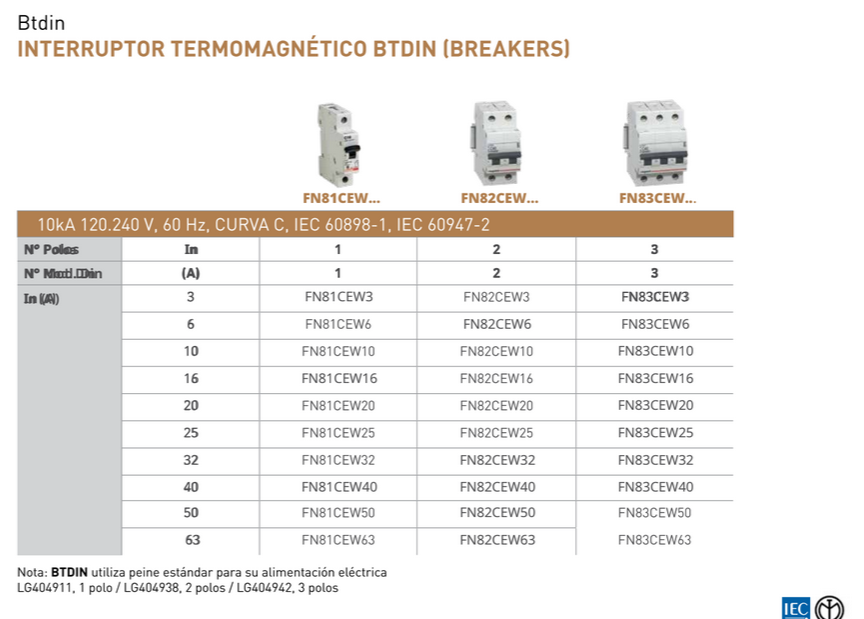
\includegraphics[width=0.75\linewidth]{images/termomagenicos del cuadro el escogido es el de 25A.png}
\caption{Interruptores termomagnéticos disponibles; el seleccionado para cada ramal es el de 25~A.}
\label{fig:termo}
\end{figure}

\subsection{Tableros de distribución por planta}

La selección del tablero de distribución para cada planta se realizó con base en el número de luminarias por nivel, reservando al menos un 30~\% de posiciones libres para circuitos de tomacorrientes y usos futuros. Los tableros disponibles son de 3, 4, 6, 8, 12, 16, 24, 36 y 42 circuitos (Figura~\ref{fig:tableros}).

\begin{figure}[H]
\centering
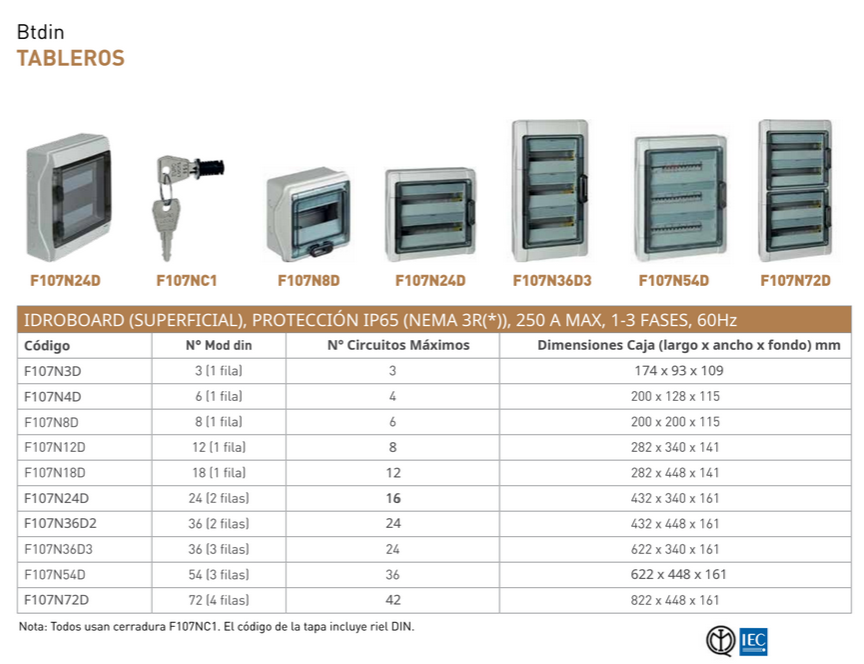
\includegraphics[width=0.85\linewidth]{images/tableros del cuadro escogido hay de 3, 4, 6, 8, 12, 16, 24, 36, 42 numero de circuitos maximo .png}
\caption{Línea de tableros de distribución disponibles (3 a 42 circuitos); referencia utilizada para la selección por planta.}
\label{fig:tableros}
\end{figure}

La Tabla~\ref{tab:tableros} resume la selección y su justificación.

\begin{table}[H]
\centering
\caption{Selección de tablero de distribución por planta.}
\label{tab:tableros}
\begin{tabular}{lcccp{2.8cm}}
\toprule
\textbf{Planta} & \textbf{Lum.} & \textbf{Circ. ilum.} & \textbf{Tablero} & \textbf{Justificación} \\
\midrule
Primer piso    & 17 & 17 & 24 circ. & 17 breakers + 7 libres para tomacorrientes y reserva \\
Segundo piso   & 14 & 14 & 16 circ. & 14 breakers + 2 libres de reserva \\
Tercer piso    &  9 &  9 & 12 circ. & 9 breakers + 3 libres para expansión \\
Planta techos  &  4 &  4 &  6 circ. & 4 breakers + 2 libres para reserva \\
\bottomrule
\end{tabular}
\end{table}

Se aclara que en este diseño cada luminaria constituye un circuito ramal independiente, lo que maximiza la selectividad: la apertura de un termomagnético afecta únicamente a la luminaria correspondiente, sin propagar el apagado a los demás puntos de luz de la planta. Esta sectorización, aunque implica mayor número de breakers, es la práctica más robusta desde el punto de vista de continuidad del servicio y facilidad de mantenimiento.

%% ─── Conclusiones ───────────────────────────────────────────────────────────
\section{Conclusiones}

\begin{itemize}
  \item El levantamiento de los planos arquitectónicos permitió cuantificar la carga de iluminación proyectada en 44 luminarias de $240~\Omega$, distribuidas en cuatro plantas con una densidad promedio de $\approx 1$ punto de luz cada 6~m².

  \item La topología serie con 44 elementos en cadena resulta inviable para iluminación funcional: cada lámpara recibe únicamente 2{,}73~V ($2{,}3\%$ del nominal) y disipa 30{,}9~mW, quedando prácticamente apagada. Adicionalmente, el fallo de un solo elemento interrumpe el suministro a las cuatro plantas en simultáneo.

  \item La topología paralelo garantiza 120~V nominales en cada luminaria, operación independiente de todas las ramas y una demanda total de 2{,}64~kW. Es la única configuración compatible con el RETIE y la NTC~2050 para instalaciones residenciales en Colombia. La demanda de 22~A justifica la sectorización en circuitos ramales de 15--20~A con protección termomagnética individual.

  \item La simulación en SimulIDE validó con error nulo los valores analíticos en ambas topologías ($V_k$, $I_{total}$, $R_{eq}$, $P_{total}$). El control automático mediante relés demostró que la lógica de mando centralizado es funcional sin alterar las condiciones eléctricas del circuito de potencia.

  \item Se recomienda ejecutar la instalación en topología paralelo, con al menos dos circuitos ramales por planta (conductor \#12~AWG, protección de 20~A), conforme a los requisitos del RETIE.
\end{itemize}

%% ─── Anexos ─────────────────────────────────────────────────────────────────
\section*{Anexos}

Los archivos complementarios de este proyecto se organizan en tres carpetas entregadas junto con el presente informe:

\medskip
\noindent\textbf{Carpeta 01\_Investigacion}
\begin{itemize}
  \item \texttt{informe\_final.pdf} — presente documento en formato de entrega.
  \item Fichas técnicas completas de los elementos seleccionados para la instalación: luminaria circular 60~W, interruptor sencillo, conductor THHN \#12~AWG, interruptor termomagnético 25~A y tableros de distribución.
\end{itemize}

\medskip
\noindent\textbf{Carpeta 02\_Diseño}
\begin{itemize}
  \item Plano arquitectónico por planta en formato PDF (escala 1:50) — cuatro láminas.
  \item Plano eléctrico con conexionado serie y paralelo en formato PDF (escala 1:50).
  \item Archivo de edición \texttt{[archivo autocad de los planos].dwg} — fuente AutoCAD de todos los planos anteriores.
\end{itemize}

\medskip
\noindent\textbf{Carpeta 03\_Simulacion}
\begin{itemize}
  \item \texttt{Simulacion\_Electrica\_Luminarias.xlsx} — Libro de cálculo con el inventario de luminarias por planta y ambiente, tablas de simulación para las topologías en serie y paralelo, y un resumen comparativo de resultados.
  \item Subcarpeta \texttt{Simulacion\_Automatica/} — Archivos fuente de SimulIDE (\texttt{.simu}) para los escenarios de mando automático. Requieren tener instalado SimulIDE para abrirse; de lo contrario, remitirse al video de la simulación.
  \item Subcarpeta \texttt{Simulacion\_Manual/} — Archivos fuente de SimulIDE (\texttt{.simu}) para los escenarios de mando manual. Misma consideración anterior.
  \item \texttt{Video\_simulacion.mp4} — Video que muestra la simulación con las dos topologías (serie y paralelo). En la configuración manual se empleó un interruptor por cada luminaria, al igual que para la configuración en automático. Además, incluye una explicación del libro de cálculo con el inventario de luminarias.
\end{itemize}